%==============================================================================
\chapter{Chemische kinetiek}
\label{ch:kinetiek}
%==============================================================================

\section{Thermodynamica bepaalt, kinetiek levert}

De thermodynamica vertelt \emph{wat} mogelijk is: of een reactie spontaan verloopt en waar het evenwicht ligt. Ze zegt niets over \emph{hoe snel}. Diamant zou spontaan moeten omzetten in grafiet, maar dat gebeurt in geen mensenleven (hoofdstuk~\ref{ch:spontaniteit}). Een methanolfabriek werkt bij \SIrange{200}{300}{\celsius}, hoewel het evenwicht een lagere temperatuur zou verkiezen. En een katalysator versnelt een reactie zonder het evenwicht te verschuiven. Dat alles is het domein van de \emph{chemische kinetiek}: de snelheid van reacties en het mechanisme waarlangs ze verlopen. De activeringsenergie en de Boltzmannfactor uit hoofdstuk~\ref{ch:kwantum} (\S~\ref{sec:activeringsenergie-kwantum} en \S~\ref{sec:boltzmannverdeling}) zijn het vertrekpunt.

We bouwen op van snelheidswet en Arrhenius, via de botsingstheorie, naar wat de ingenieur het meest nodig heeft: selectiviteit, mechanismen, katalyse en de koppeling tussen reactiewarmte en snelheid. Het eigenlijke reactorontwerp volgt in Reactorentechnologie.

\begin{toepassing}{Centrale case: ethyleenoxide, selectief en veilig}
Ethyleenoxide (grondstof voor glycol, antivries en polyesters, met grote productie-eenheden in de Antwerpse haven) wordt gemaakt door ethyleen te oxideren over een zilverkatalysator bij \SIrange{220}{280}{\celsius}:
\begin{align*}
\mathrm{C_2H_4 + \tfrac12\,O_2} &\rightarrow \mathrm{C_2H_4O} && \Delta_rH^\circ \approx \SI{-105}{\kilo\joule\per\mole} \quad\text{(gewenst)},\\
\mathrm{C_2H_4 + 3\,O_2} &\rightarrow \mathrm{2\,CO_2 + 2\,H_2O} && \Delta_rH^\circ \approx \SI{-1323}{\kilo\joule\per\mole} \quad\text{(ongewenst)}.
\end{align*}
Beide reacties zijn thermodynamisch volledig: $K$ is enorm. Wat er gevormd wordt, bepaalt dus enkel de kinetiek. Elke procent ethyleen die verbrandt in plaats van epoxide te vormen, kost grondstof \'en levert twaalf keer meer warmte. Dit hoofdstuk geeft de middelen om te begrijpen waarom de temperatuur de selectiviteit bepaalt (\S~\ref{sec:selectiviteit}) en hoe die extra warmte een reactor op hol kan doen slaan (\S~\ref{sec:runaway}).
\end{toepassing}

\section{De reactiesnelheid}

Beschouw een algemene reactie:
\begin{equation}
aA + bB \rightarrow cC + dD.
\end{equation}
De \emph{reactiesnelheid} $r$ wordt gedefinieerd als de verandering van de concentratie van een component per eenheid van tijd, gecorrigeerd voor de stoichiometrie:
\begin{equation}
\boxed{\;r = -\frac{1}{a}\frac{\dd{[A]}}{\dd{t}} = -\frac{1}{b}\frac{\dd{[B]}}{\dd{t}} = \frac{1}{c}\frac{\dd{[C]}}{\dd{t}} = \frac{1}{d}\frac{\dd{[D]}}{\dd{t}}\;}
\end{equation}
Het minteken voor de reactanten zorgt ervoor dat $r$ steeds positief is. De stoichiometrische co\"effici\"enten in de noemer garanderen dat $r$ onafhankelijk is van de gekozen component.

\begin{voorbeeld}{Snelheid van de ammoniaksynthese}
Voor $\mathrm{N_2 + 3\,H_2 \rightarrow 2\,NH_3}$ geldt:
\[
r = -\frac{\dd{[\mathrm{N_2}]}}{\dd{t}} = -\frac{1}{3}\frac{\dd{[\mathrm{H_2}]}}{\dd{t}} = \frac{1}{2}\frac{\dd{[\mathrm{NH_3}]}}{\dd{t}}.
\]
Wanneer \SI{0.5}{\mole\per\litre\per\second} van $\mathrm{N_2}$ wordt omgezet, wordt $\mathrm{H_2}$ driemaal sneller verbruikt en $\mathrm{NH_3}$ tweemaal sneller gevormd. De snelheid $r$ is echter voor alle componenten gelijk: $r = \SI{0.5}{\mole\per\litre\per\second}$.
\end{voorbeeld}

\section{De snelheidswet: invloed van de concentratie}
\label{sec:snelheidswet}

Experimenteel wordt vastgesteld dat de reactiesnelheid vaak afhangt van de concentraties van de reactanten. Voor vele reacties geldt een \emph{machtswet}:
\begin{equation}
\boxed{\;r = k\,[A]^m\,[B]^n\;}
\end{equation}
waarin $k$ de \emph{snelheidsconstante}, $m$ de reactieorde met betrekking tot $A$ en $n$ de reactieorde met betrekking tot $B$ voorstellen. De som $m+n$ is de \emph{totale reactieorde}. De reactieorde is in het algemeen \emph{geen} geheel getal en hoeft niet overeen te komen met de stoichiometrische co\"effici\"enten: zij moet experimenteel worden bepaald.

\subsection{Nulde-orde reacties}

Voor een nulde-orde reactie ($m=0$) geldt:
\begin{equation}
r = k.
\end{equation}
De snelheid is onafhankelijk van de concentratie. Integratie levert:
\begin{equation}
[A](t) = [A]_0 - k\,t.
\label{eq:nulde-orde}
\end{equation}
De concentratie neemt lineair af met de tijd. De halfwaardetijd bedraagt $t_{1/2} = [A]_0/(2k)$. Nulde-orde gedrag treedt op bij oppervlaktereacties met een verzadigd oppervlak (\S~\ref{sec:langmuir-isotherm-kinetiek}) of enzymreacties bij verzadiging (\S~\ref{sec:michaelis-menten}).

\subsection{Eerste-orde reacties}

Voor een eerste-orde reactie ($m=1$) geldt:
\begin{equation}
r = -\frac{\dd{[A]}}{\dd{t}} = k\,[A].
\end{equation}
Integratie levert:
\begin{equation}
\boxed{\;\ln\frac{[A]_0}{[A]} = k\,t \;\;\Leftrightarrow\;\; [A](t) = [A]_0\,e^{-kt}\;}
\label{eq:eerste-orde}
\end{equation}
De halfwaardetijd is onafhankelijk van de beginconcentratie:
\begin{equation}
\boxed{\;t_{1/2} = \frac{\ln 2}{k}\;}
\end{equation}
Eerste-orde reacties zijn het meest voorkomende type: radioactief verval, thermische ontleding van vele verbindingen, en de meeste enzymreacties in hun initi\"ele stadia volgen eerste-orde kinetiek. In \S~\ref{sec:lindemann} zullen we zien dat zelfs een reactie die conceptueel ``\'e\'en molecule valt uit elkaar'' betekent, niet noodzakelijk overal eerste-orde gedrag vertoont.

\begin{voorbeeld}{Thermische ontleding van $\mathrm{N_2O_5}$}
De ontleding van distikstofpentoxide:
\[
\mathrm{2\,N_2O_5(g) \rightarrow 4\,NO_2(g) + O_2(g)}
\]
verloopt volgens eerste-orde kinetiek. Bij \SI{300}{\kelvin} bedraagt $k = \SI{3.4e-5}{\per\second}$. De halfwaardetijd is:
\[
t_{1/2} = \frac{\ln 2}{k} = \frac{0.693}{\SI{3.4e-5}{\per\second}} \approx \SI{20000}{\second} \approx \SI{5.6}{\hour}.
\]
Na \SI{5.6}{\hour} is de helft van de beginconcentratie omgezet, ongeacht de beginwaarde.
\end{voorbeeld}

\subsection{Tweede-orde reacties}

Voor een tweede-orde reactie ($m=2$ of $m=1, n=1$) geldt:
\begin{equation}
r = k\,[A]^2.
\end{equation}
Integratie levert:
\begin{equation}
\boxed{\;\frac{1}{[A]} - \frac{1}{[A]_0} = k\,t\;}
\label{eq:tweede-orde}
\end{equation}
De halfwaardetijd is nu \emph{wel} afhankelijk van de beginconcentratie:
\begin{equation}
t_{1/2} = \frac{1}{k\,[A]_0}.
\label{eq:thalf-tweede}
\end{equation}
Hoe hoger de beginconcentratie, hoe korter de halfwaardetijd. Veel bimoleculaire reacties in oplossing (neutralisatiereacties, condensatiereacties) volgen tweede-orde kinetiek.

\begin{figure}[htb]
    \centering
    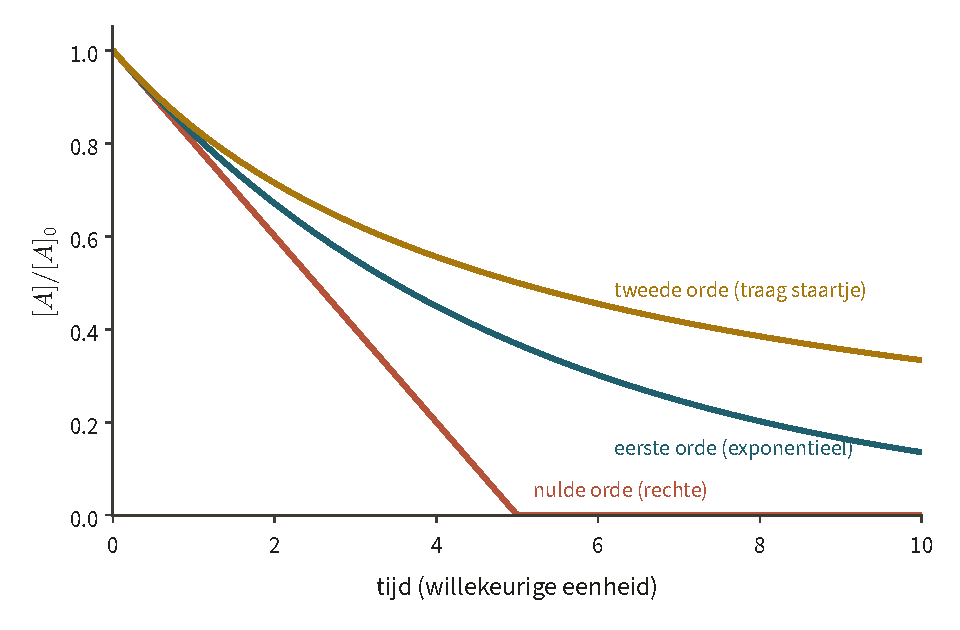
\includegraphics[width=0.7\linewidth]{Figuren/ordes}
    \caption{Concentratieverloop voor een nulde-, eerste- en tweede-orde reactie met dezelfde beginconcentratie en dezelfde beginsnelheid. Een rechte (nulde orde), een exponenti\"ele daling (eerste orde) en een trage staart (tweede orde): de integratiemethode maakt van dit verschil gebruik.}
    \label{fig:ordes-concentratie-tijd}
\end{figure}

\subsection{Bepaling van de reactieorde}
\label{sec:bepaling-orde}

De reactieorde kan experimenteel worden bepaald door:
\begin{itemize}
\item \textbf{De integratiemethode}: test of $\ln[A]$, $1/[A]$ of $[A]$ lineair verloopt met de tijd (figuur~\ref{fig:ordes-concentratie-tijd}).
\item \textbf{De isolatiemethode}: houd alle reactanten behalve \'e\'en in groot overschot, zodat hun concentratie constant is. De reactieorde met betrekking tot de vari\"erende component wordt zo ge\"isoleerd.
\item \textbf{De methode van initi\"ele snelheden}: meet $r$ aanvankelijk voor verschillende beginconcentraties en vergelijk $\log r$ met $\log[A]$.
\end{itemize}

\section{De invloed van temperatuur: de vergelijking van Arrhenius}
\label{sec:arrhenius}

Voor nagenoeg alle chemische reacties neemt de reactiesnelheid sterk toe met de temperatuur. Een ruwe vuistregel: per \SI{10}{\kelvin} verdubbelt de snelheid. Kwantitatief geldt de \emph{vergelijking van Arrhenius}:
\begin{equation}
\boxed{\;k = A\,\exp\!\left(-\frac{E_a}{RT}\right)\;}
\label{eq:arrhenius}
\end{equation}
met $A$ de \emph{pre\"exponenti\"ele factor} en $E_a$ de \emph{activeringsenergie}, de energiedrempel tussen reagentia en overgangstoestand (\S~\ref{sec:activeringsenergie-kwantum}). De exponenti\"ele vorm verklaart waarom de snelheid zo sterk met de temperatuur stijgt: een verhoging van $T$ verhoogt de fractie van de moleculen met voldoende energie om de activeringsdrempel te overschrijden. Merk meteen op dat deze fractie, en dus de \emph{gevoeligheid} van $k$ voor temperatuur, sterker is naarmate $E_a$ groter is --- een inzicht dat we in \S~\ref{sec:temperatuursgevoeligheid} kwantitatief zullen uitwerken.

\subsection{De betekenis van de activeringsenergie}

De activeringsenergie $E_a$ is de minimale energie die een molecule (of een paar botsende moleculen) moet bezitten om de reactie te laten plaatsvinden. Uit de vergelijking van Arrhenius volgt:
\begin{equation}
\ln k = \ln A - \frac{E_a}{RT}.
\label{eq:arrhenius-log}
\end{equation}
Door $\ln k$ uit te zetten tegen $1/T$ ontstaat een rechte met helling $-E_a/R$. Dit is de \emph{Arrhenius-grafiek}, waarmee $E_a$ uit experimentele snelheidsmetingen bij verschillende temperaturen kan worden bepaald.

\begin{figure}[htb]
    \centering
    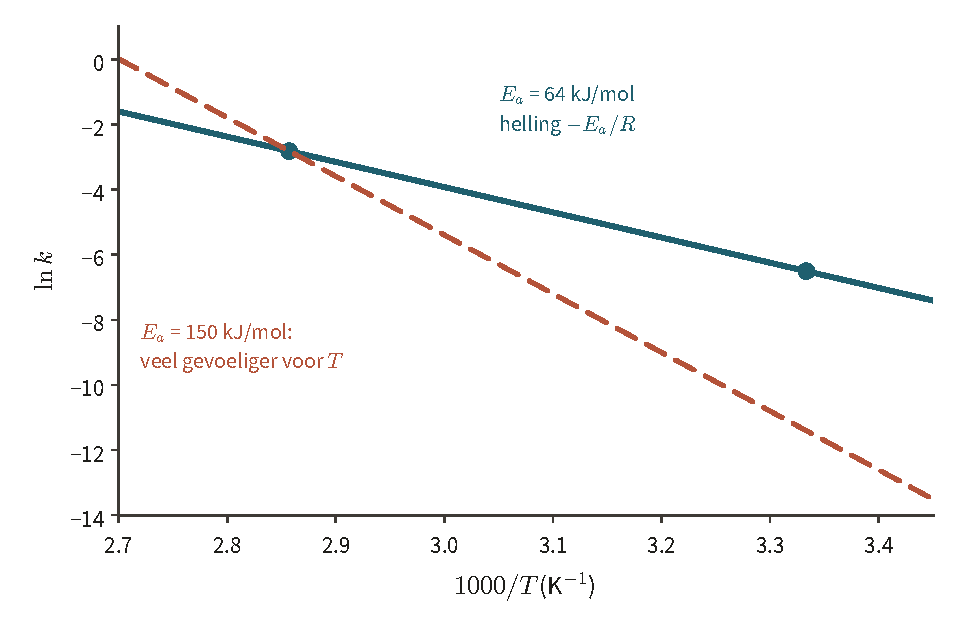
\includegraphics[width=0.7\linewidth]{Figuren/arrhenius}
    \caption{Arrheniusgrafiek: $\ln k$ tegen $1/T$ geeft een rechte met helling $-E_a/R$. De punten zijn de twee metingen uit het voorbeeld hieronder. De stippellijn is een reactie met een hogere activeringsenergie: ze is veel gevoeliger voor de temperatuur.}
    \label{fig:arrhenius-grafiek}
\end{figure}

\begin{voorbeeld}{Bepaling van $E_a$ uit twee metingen}
Voor een bepaalde reactie is $k = \SI{1.5e-3}{\per\second}$ bij \SI{300}{\kelvin} en $k = \SI{6.0e-2}{\per\second}$ bij \SI{350}{\kelvin}. Uit de ge\"integreerde Arrheniusvergelijking (volledig analoog aan de ge\"integreerde vergelijking van Van 't Hoff, hoofdstuk~\ref{ch:reagerend}):
\[
\ln\frac{k_2}{k_1} = -\frac{E_a}{R}\left(\frac{1}{T_2} - \frac{1}{T_1}\right)
\]
volgt:
\[
E_a = -R\,\frac{\ln(k_2/k_1)}{(1/T_2 - 1/T_1)} = -(\SI{8.314}{\joule\per\mole\per\kelvin})\frac{\ln(40)}{1/350 - 1/300} \approx \SI{64.4}{\kilo\joule\per\mole}.
\]
Een activeringsenergie van \SI{64}{\kilo\joule\per\mole} is typisch voor vele thermisch geactiveerde reacties.
\end{voorbeeld}

\interactief{arrhenius}

\subsection{Temperatuurverhoging bij ammoniaksynthese}
\label{sec:ammoniak-arrhenius}

Voor de ammoniaksynthese geldt $E_a \approx \SI{230}{\kilo\joule\per\mole}$ (zeer hoog wegens de sterke drievoudige stikstofbinding, hoofdstuk~\ref{ch:kwantum}). Een verhoging van \SI{300}{\kelvin} naar \SI{700}{\kelvin} levert:
\[
\frac{k(700)}{k(300)} = \exp\left[-\frac{230\,000}{8.314}\left(\frac{1}{700} - \frac{1}{300}\right)\right] \approx 7.7\times10^{22}.
\]
De reactiesnelheid neemt astronomisch toe. Dit verklaart waarom het Haber--Boschproces ondanks de thermodynamisch ongunstige hoge temperatuur toch bij \SIrange{400}{500}{\celsius} wordt uitgevoerd (hoofdstuk~\ref{ch:reagerend}, \S~\ref{sec:haber-bosch-integraal}): zonder voldoende temperatuur zou de kinetiek het proces volledig onmogelijk maken, ondanks de thermodynamische gunst bij lage temperatuur. We komen op dit precieze getal terug in \S~\ref{sec:temperatuursgevoeligheid}, waar we het vergelijken met de temperatuursgevoeligheid van de \emph{teruggaande} reactie.

\section{Waarom Arrhenius? De botsingstheorie}
\label{sec:botsingstheorie}

De vergelijking van Arrhenius is empirisch. Voor gasreacties kunnen we haar begrijpen met de kinetische gastheorie van hoofdstuk~\ref{ch:energie} (\S~\ref{sec:kinetische-gastheorie}): twee moleculen kunnen pas reageren als ze botsen, en enkel als die botsing hard genoeg is.

\subsection{Snelheden, botsingen en vrije weglengte}

De moleculen in een gas hebben niet allemaal dezelfde snelheid. De verdeling volgt uit de Boltzmannfactor (hoofdstuk~\ref{ch:kwantum}, \S~\ref{sec:boltzmannverdeling}) toegepast op de kinetische energie $\tfrac12 mv^2$; ze heet de \emph{Maxwell--Boltzmannverdeling}:
\begin{equation}
f(v) = 4\pi\left(\frac{M}{2\pi RT}\right)^{3/2} v^2\,\exp\!\left(-\frac{Mv^2}{2RT}\right),
\qquad
\bar v = \sqrt{\frac{8RT}{\pi M}}.
\label{eq:maxwell-boltzmann}
\end{equation}
De factor $v^2$ telt het aantal richtingen waarin een molecule met snelheid $v$ kan bewegen; de exponenti\"ele factor maakt hoge snelheden zeldzaam. Bij hogere temperatuur schuift de verdeling op en wordt ze breder (figuur~\ref{fig:maxwell-boltzmann}). Vooral de staart met zeer snelle moleculen groeit sterk: daar zitten de moleculen die kunnen reageren.

\begin{figure}[htb]
    \centering
    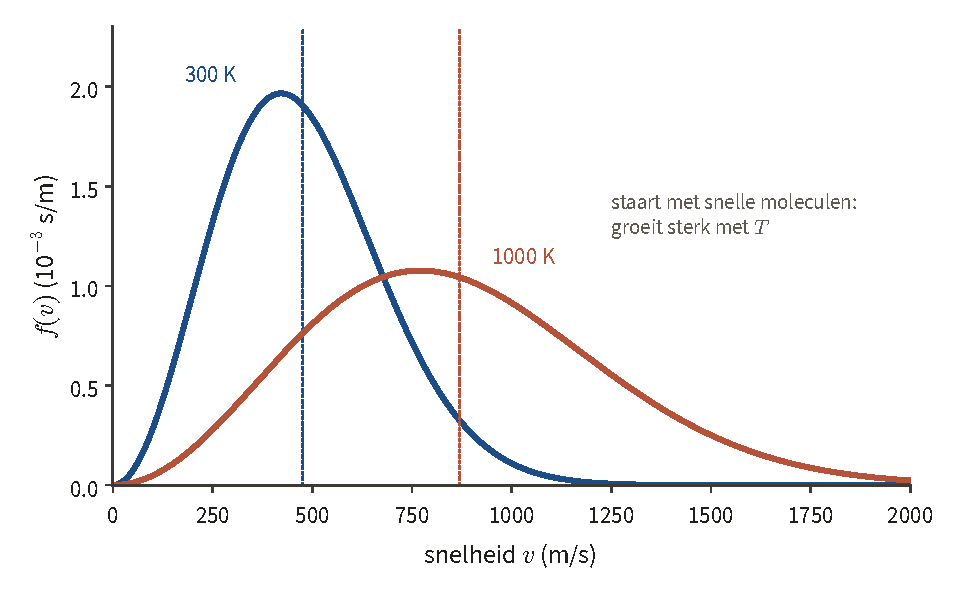
\includegraphics[width=0.7\linewidth]{Figuren/maxwell_boltzmann}
    \caption{Maxwell--Boltzmannverdeling van de snelheid van N$_2$ bij \SI{300}{\kelvin} en \SI{1000}{\kelvin}. De stippellijnen geven de gemiddelde snelheid $\bar v$.}
    \label{fig:maxwell-boltzmann}
\end{figure}

Een molecule met diameter $d$ botst met elk ander molecule waarvan het centrum binnen een cilinder met doorsnede $\sigma = \pi d^2$ (de \emph{botsingsdoorsnede}) ligt. Daaruit volgen de \emph{botsingsfrequentie} van \'e\'en molecule en de gemiddelde afstand tussen twee botsingen, de \emph{vrije weglengte}:
\begin{equation}
z = \sqrt2\,\sigma\,\bar v\,\frac{p}{k_BT},
\qquad
\lambda = \frac{\bar v}{z} = \frac{k_BT}{\sqrt2\,\sigma\,p}.
\label{eq:vrije-weglengte}
\end{equation}
De factor $\sqrt2$ komt van de relatieve snelheid tussen twee bewegende moleculen.

\begin{voorbeeld}{Stikstof bij kamertemperatuur}
Voor N$_2$ bij \SI{298}{\kelvin} en \SI{1}{\bar} is $\sigma \approx \SI{0.43}{\nano\metre\squared}$ en $\bar v = \sqrt{8(8.314)(298)/(\pi\cdot0.028)} = \SI{475}{\metre\per\second}$. Dan is
\[
\lambda = \frac{(\SI{1.381e-23}{})(298)}{\sqrt2\,(\SI{0.43e-18}{})(\SI{1e5}{})} = \SI{68}{\nano\metre},
\qquad
z = \frac{\bar v}{\lambda} = \SI{7e9}{\per\second}.
\]
Elke molecule botst zeven miljard keer per seconde, en legt tussen twee botsingen een afstand af van ongeveer tweehonderd keer haar eigen diameter.
\end{voorbeeld}

\begin{toepassing}{Vacuüm, poriën en isotopen: drie praktische haakjes}
\begin{itemize}
\item \textbf{Vacuümtechniek.} De vrije weglengte is omgekeerd evenredig met de druk. Bij \SI{e-6}{\milli\bar} (\SI{e-4}{\pascal}), typisch voor een coatingkamer of elektronenmicroscoop, is $\lambda \approx \SI{70}{\metre}$: moleculen botsen enkel nog tegen de wanden. Men spreekt van \emph{moleculaire stroming}, en de pompsnelheid wordt dan bepaald door de opening en niet meer door de viscositeit van het gas.
\item \textbf{Knudsendiffusie.} Is de vrije weglengte groter dan de poriediameter $d_p$ (het \emph{Knudsengetal} $\mathrm{Kn} = \lambda/d_p > 1$), dan botsen moleculen vaker met de wand dan met elkaar. In de poriën van \SI{10}{\nano\metre} van de katalysatorkorrel uit hoofdstuk~\ref{ch:grensvlakken} is dat al zo bij \SI{1}{\bar}. De diffusieco\"effici\"ent hangt dan af van $\bar v$ en de poriegrootte, niet van de druk.
\item \textbf{Effusie.} Door een gaatje dat kleiner is dan $\lambda$ ontsnappen moleculen met een snelheid evenredig met $\bar v \propto 1/\sqrt{M}$: de wet van Graham uit hoofdstuk~\ref{ch:energie}.
\end{itemize}
\end{toepassing}

\subsection{Van botsing naar reactie}

Niet elke botsing leidt tot een reactie. Twee voorwaarden moeten vervuld zijn:
\begin{enumerate}
\item De botsing moet genoeg energie hebben: de kinetische energie langs de verbindingslijn van beide centra moet minstens $E_a$ zijn. De fractie botsingen die daaraan voldoet, is precies de Boltzmannfactor $\exp(-E_a/RT)$.
\item De moleculen moeten juist gericht zijn. Bij grote moleculen leidt enkel een klein deel van de botsingen tot reactie. Dat deel heet de \emph{sterische factor} $P$.
\end{enumerate}
Het aantal botsingen per volume en per tijd tussen A en B is $\sigma\,\bar v_\mathrm{rel}\,N_A^2[A][B]$, met $\bar v_\mathrm{rel} = \sqrt{8RT/\pi\mu}$ en $\mu$ de gereduceerde molaire massa. Vermenigvuldigen met beide fracties geeft de snelheidsconstante:
\begin{equation}
\boxed{\;k = P\,\sigma\,\bar v_\mathrm{rel}\,N_A\,\exp\!\left(-\frac{E_a}{RT}\right)\;}
\label{eq:botsingstheorie}
\end{equation}
Dat is de vergelijking van Arrhenius, met een pre\"exponenti\"ele factor $A = P\,\sigma\,\bar v_\mathrm{rel}\,N_A$. De exponenti\"ele factor bevat bijna alle temperatuursafhankelijkheid; $A$ stijgt slechts met $\sqrt T$.

\begin{voorbeeld}{Hoe groot kan $A$ zijn?}
Voor twee moleculen zo groot als N$_2$ ($\sigma = \SI{0.43}{\nano\metre\squared}$, $\bar v_\mathrm{rel} = \sqrt2\cdot\SI{475}{\metre\per\second} = \SI{672}{\metre\per\second}$) bij kamertemperatuur:
\begin{align*}
A = \sigma\,\bar v_\mathrm{rel}\,N_A &= (\SI{0.43e-18}{\metre\squared})(\SI{672}{\metre\per\second})(\SI{6.022e23}{\per\mole})\\
&= \SI{1.7e8}{\metre\cubed\per\mole\per\second} = \SI{1.7e11}{\litre\per\mole\per\second}.
\end{align*}
Gemeten waarden voor eenvoudige radicaalreacties liggen in die buurt ($P \approx 0.1$--1). Voor reacties tussen grote organische moleculen meet men vaak $10^{-3}$ tot $10^{-6}$ keer minder: de sterische factor is dan klein, omdat slechts een klein stukje van elk molecule reactief is.
\end{voorbeeld}

De botsingstheorie verklaart dus waarom $\ln k$ lineair daalt met $1/T$, en waarom een hogere activeringsenergie een sterkere temperatuursafhankelijkheid geeft. Voor reacties in oplossing en op oppervlakken is het beeld minder eenvoudig, maar de Boltzmannfactor blijft de kern.

\section{Omkeerbare en concurrerende reacties}
\label{sec:meervoudige-reacties}

Industri\"ele reacties verlopen zelden alleen. Het product kan terugreageren, de grondstof kan op meer dan \'e\'en manier reageren, en het gewenste product kan zelf verder reageren. Voor de ingenieur is niet alleen de \emph{omzetting} $X$ belangrijk, maar vooral de \emph{selectiviteit} $S$ (welk deel van de omgezette grondstof wordt gewenst product) en de \emph{opbrengst} $Y = X\,S$.

\subsection{Omkeerbare reacties: de weg naar evenwicht}
\label{sec:omkeerbare-reacties}

Voor $A \rightleftharpoons B$ met eerste-orde snelheidsconstanten $k_1$ (heen) en $k_{-1}$ (terug) geldt
\[
-\frac{\dd{[A]}}{\dd{t}} = k_1[A] - k_{-1}[B].
\]
In evenwicht is de netto snelheid nul: $K = [B]_\mathrm{eq}/[A]_\mathrm{eq} = k_1/k_{-1}$. Dit is dezelfde $K$ als in hoofdstuk~\ref{ch:reagerend}. Integratie geeft
\begin{equation}
[A] - [A]_\mathrm{eq} = \bigl([A]_0 - [A]_\mathrm{eq}\bigr)\,e^{-(k_1+k_{-1})t}.
\label{eq:relaxatie}
\end{equation}
Het systeem nadert het evenwicht exponentieel, met een karakteristieke tijd $1/(k_1+k_{-1})$: de \emph{som} van beide snelheidsconstanten, niet $k_1$ alleen. De thermodynamica (via $K$) zegt waar de reactie eindigt; de kinetiek zegt hoe snel. In \S~\ref{sec:brug-thermo-kinetiek} volgt hieruit een verband tussen de activeringsenergie\"en en $\Delta_rH^\circ$.

\subsection{Parallelle reacties en selectiviteit}
\label{sec:selectiviteit}

Bij twee \emph{parallelle} reacties uit dezelfde grondstof,
\[
A \xrightarrow{k_1} B \ \text{(gewenst)}, \qquad A \xrightarrow{k_2} C \ \text{(ongewenst)},
\]
met dezelfde orde in $A$, is de verhouding van de vormingssnelheden constant, en de selectiviteit
\begin{equation}
S = \frac{k_1}{k_1 + k_2} = \frac{1}{1 + \dfrac{A_2}{A_1}\exp\!\left(-\dfrac{E_{a,2} - E_{a,1}}{RT}\right)}.
\label{eq:selectiviteit}
\end{equation}
De temperatuur werkt dus in het voordeel van de reactie met de \emph{hoogste} activeringsenergie. Twee regels volgen meteen:
\begin{itemize}
\item Heeft de gewenste reactie de laagste $E_a$, dan geeft een lage temperatuur een betere selectiviteit, maar een tragere reactie. Een selectieve katalysator verlaagt vooral $E_{a,1}$.
\item Verschillen de reactieordes, dan speelt ook de concentratie mee: is de gewenste reactie van hogere orde in $A$, dan houdt men $[A]$ hoog (batch- of propstroomreactor); is ze van lagere orde, dan werkt men verdund (geroerde tank, CSTR).
\end{itemize}

\begin{voorbeeld}{Ethyleenoxide: selectiviteit en temperatuur}
Neem voor de centrale case $E_{a,1} \approx \SI{60}{\kilo\joule\per\mole}$ voor de epoxidering en $E_{a,2} \approx \SI{80}{\kilo\joule\per\mole}$ voor de volledige verbranding (illustratieve waarden), en kies $A_2/A_1$ zo dat $S = 0.85$ bij \SI{500}{\kelvin}. Met vergelijking~\eqref{eq:selectiviteit}:
\begin{center}
\begin{tabular}{lccc}
\toprule
$T$ (K) & 470 & 500 & 550 \\
\midrule
$S$ & 0.885 & 0.85 & 0.79 \\
warmte per mol omgezet ethyleen (kJ) & 245 & 288 & 366 \\
\bottomrule
\end{tabular}
\end{center}
De warmte is $S(105) + (1-S)(1323)$~kJ. Vijftig graden warmer kost zes procentpunten selectiviteit en levert een kwart meer warmte. Die extra warmte maakt de reactor nog warmer, wat de selectiviteit verder verlaagt: een gevaarlijke terugkoppeling (\S~\ref{sec:runaway}). Daarom bewaakt men de temperatuur van een EO-reactor tot op enkele graden en voegt men kleine hoeveelheden gechloreerde moderatoren toe die de verbranding sterker afremmen dan de epoxidering.
\end{voorbeeld}

\subsection{Reacties in serie: het tussenproduct}
\label{sec:serie-reacties}

Vaak is het gewenste product zelf reactief: $A \xrightarrow{k_1} B \xrightarrow{k_2} C$. Denk aan de gedeeltelijke oxidatie van koolwaterstoffen, waar het product verder verbrandt, of aan een geneesmiddel dat in het lichaam wordt omgezet tot een actieve vorm en daarna afgebroken. Met eerste-orde kinetiek en enkel $A$ bij de start volgt
\begin{equation}
[A] = [A]_0\,e^{-k_1t},
\qquad
[B] = [A]_0\,\frac{k_1}{k_2-k_1}\bigl(e^{-k_1t} - e^{-k_2t}\bigr).
\label{eq:serie}
\end{equation}
Het tussenproduct stijgt eerst, bereikt een maximum en verdwijnt dan (figuur~\ref{fig:serie-reactie}). Afleiden van $[B]$ naar $t$ en gelijkstellen aan nul geeft het optimum:
\begin{equation}
\boxed{\;t_\mathrm{max} = \frac{\ln(k_2/k_1)}{k_2-k_1},
\qquad
\frac{[B]_\mathrm{max}}{[A]_0} = \left(\frac{k_1}{k_2}\right)^{k_2/(k_2-k_1)}\;}
\label{eq:serie-max}
\end{equation}

\begin{figure}[htb]
    \centering
    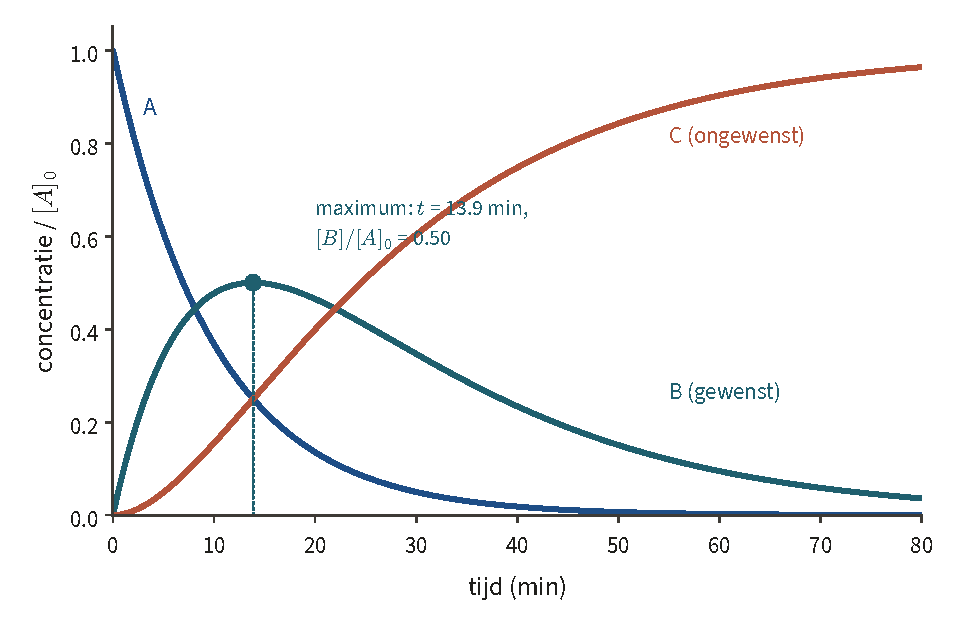
\includegraphics[width=0.7\linewidth]{Figuren/serie_reactie}
    \caption{Reacties in serie $A \to B \to C$ met $k_1 = \SI{0.10}{\per\minute}$ en $k_2 = \SI{0.05}{\per\minute}$. Het tussenproduct $B$ bereikt een maximum; wie te lang wacht, verliest het gewenste product.}
    \label{fig:serie-reactie}
\end{figure}

Voor $k_1 = \SI{0.10}{\per\minute}$ en $k_2 = \SI{0.05}{\per\minute}$ is $t_\mathrm{max} = \ln 0.5/(-0.05) = \SI{13.9}{\minute}$ en $[B]_\mathrm{max} = 0.50\,[A]_0$. De les voor de ingenieur: bij reacties in serie is maximale omzetting \emph{niet} het doel. Men stopt de batch op het juiste moment, of kiest in een continue reactor de verblijftijd zo dat de opbrengst aan $B$ maximaal is, en recycleert de niet-omgezette $A$.

\section{Reactiemechanismen en elementaire reacties}
\label{sec:mechanismen}

Bijna geen enkele reactie verloopt in \'e\'en stap. De brutoreactie beschrijft enkel begin- en eindtoestand; de weg ertussen is het \emph{reactiemechanisme}, een reeks \emph{elementaire reacties}. Een elementaire reactie is \'e\'en moleculaire gebeurtenis: een molecule die uiteenvalt (\emph{unimoleculair}), twee moleculen die botsen (\emph{bimoleculair}) of, zelden, drie tegelijk (\emph{termoleculair}). Alleen voor elementaire reacties volgt de orde uit de stoichiometrie: $A + B \rightarrow P$ is dan altijd $r = k[A][B]$.

Een klassiek voorbeeld is $\mathrm{H_2 + Br_2 \rightarrow 2\,HBr}$. De reactie verloopt via een radicaalketen:
\begin{align*}
&\text{initiatie:} && \mathrm{Br_2} \rightarrow 2\,\mathrm{Br\cdot}\\
&\text{propagatie:} && \mathrm{Br\cdot + H_2} \rightarrow \mathrm{HBr + H\cdot}, \qquad \mathrm{H\cdot + Br_2} \rightarrow \mathrm{HBr + Br\cdot}\\
&\text{terminatie:} && 2\,\mathrm{Br\cdot} \rightarrow \mathrm{Br_2}
\end{align*}
met als gemeten snelheidswet $r = k[\mathrm{H_2}][\mathrm{Br_2}]^{1/2}/(1 + k'[\mathrm{HBr}]/[\mathrm{Br_2}])$. Die vorm volgt nooit uit de brutovergelijking; je hebt het mechanisme nodig.

\section{De steady-state-benadering}
\label{sec:steady-state}

Reactieve tussenproducten (radicalen, een enzym-substraatcomplex, een geactiveerde molecule) worden even snel verbruikt als gevormd. Hun concentratie blijft klein en nagenoeg constant. De \emph{steady-state-benadering} (Bodenstein) stelt daarom
\begin{equation}
\frac{\dd{[\text{tussenproduct}]}}{\dd{t}} \approx 0 .
\end{equation}
Is \'e\'en stap veel trager dan de rest, dan bepaalt die \emph{snelheidsbepalende stap} de globale snelheid, zoals de smalste flessenhals de doorstroming bepaalt.

\subsection{Voorbeeld: ontleding van ozon}
\label{sec:ozon}

$\mathrm{2\,O_3 \rightarrow 3\,O_2}$ verloopt via een snel evenwicht $\mathrm{O_3} \rightleftharpoons \mathrm{O_2 + O}$ ($k_1$, $k_{-1}$) en een trage stap $\mathrm{O + O_3} \rightarrow 2\,\mathrm{O_2}$ ($k_2$). Steady state voor het zuurstofatoom:
\[
k_1[\mathrm{O_3}] - k_{-1}[\mathrm{O_2}][\mathrm{O}] - k_2[\mathrm{O}][\mathrm{O_3}] = 0 .
\]
Omdat de tweede stap traag is ($k_2[\mathrm{O_3}] \ll k_{-1}[\mathrm{O_2}]$), volgt
\[
[\mathrm{O}] \approx \frac{k_1[\mathrm{O_3}]}{k_{-1}[\mathrm{O_2}]},
\qquad
r = k_2[\mathrm{O}][\mathrm{O_3}] = \frac{k_1 k_2}{k_{-1}} \frac{[\mathrm{O_3}]^2}{[\mathrm{O_2}]}.
\]
Het product \ce{O2} remt de reactie: iets wat je uit de brutovergelijking nooit zou raden.

\subsection{Het Lindemann-mechanisme}
\label{sec:lindemann}

Een molecule die ``gewoon uit elkaar valt'' ($A \to P$), gedraagt zich bij hoge druk als eerste orde, maar bij lage druk als tweede orde. Lindemann (1922) verklaarde dat: de molecule moet eerst energie krijgen door een botsing, en kan die bij een volgende botsing weer verliezen:
\[
A + A \xrightleftharpoons[k_{-1}]{k_1} A^* + A, \qquad A^* \xrightarrow{k_2} P .
\]
Steady state voor $A^*$ geeft $[A^*] = k_1[A]^2/(k_{-1}[A]+k_2)$, en met $r = k_2[A^*]$:
\begin{equation}
\boxed{\;r = \frac{k_1k_2[A]^2}{k_{-1}[A]+k_2}\;}
\label{eq:lindemann}
\end{equation}
Bij \textbf{hoge druk} ($k_{-1}[A] \gg k_2$) wordt een geactiveerde molecule meestal eerst weer gedeactiveerd: $r \approx (k_1k_2/k_{-1})[A]$, eerste orde. Bij \textbf{lage druk} ($k_2 \gg k_{-1}[A]$) reageert elke geactiveerde molecule meteen: $r \approx k_1[A]^2$, tweede orde, want de activerende botsing is nu de flessenhals (figuur~\ref{fig:lindemann}).

\begin{figure}[htb]
    \centering
    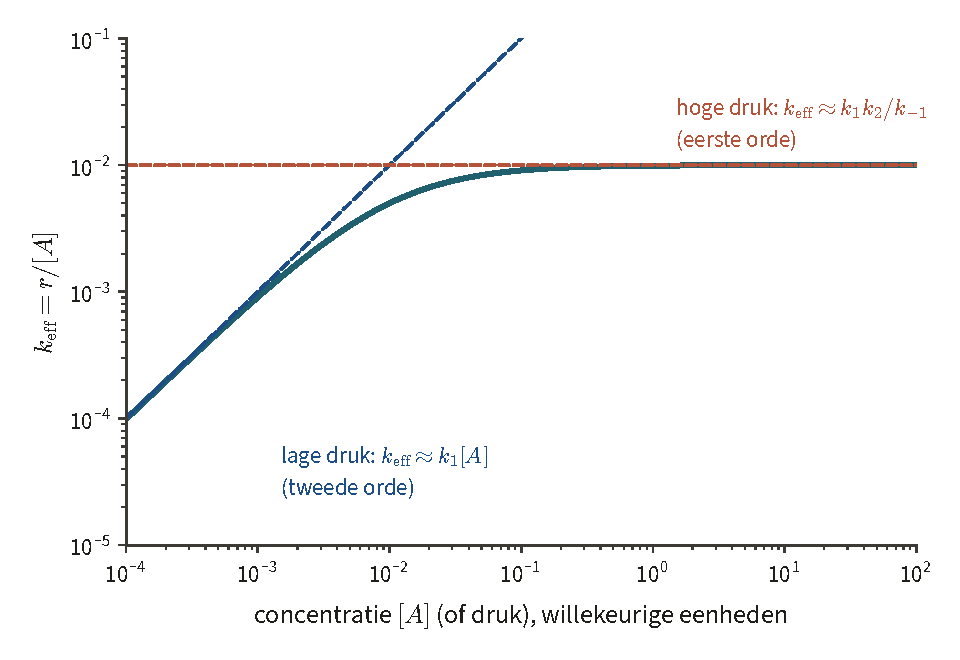
\includegraphics[width=0.7\linewidth]{Figuren/lindemann}
    \caption{Lindemann-mechanisme: de effectieve eerste-ordeconstante $k_\text{eff} = r/[A]$ in functie van de concentratie (logaritmische assen). Bij lage druk stijgt $k_\text{eff}$ evenredig met $[A]$ (tweede orde), bij hoge druk vlakt ze af tot $k_1k_2/k_{-1}$ (eerste orde). Michaelis--Menten en Langmuir--Hinshelwood tonen dezelfde verzadiging.}
    \label{fig:lindemann}
\end{figure}

Dit patroon (een orde die verschuift doordat een tussenstap verzadigt) komt verderop nog twee keer terug: bij enzymen (\S~\ref{sec:michaelis-menten}) en bij katalysatoroppervlakken (\S~\ref{sec:langmuir-hinshelwood}).

\section{Katalyse}
\label{sec:katalyse}

Een \emph{katalysator} verhoogt de reactiesnelheid zonder zelf verbruikt te worden. Hij verlaagt de activeringsenergie van heen- \'en terugreactie evenveel, zodat de evenwichtsconstante niet verandert (hoofdstuk~\ref{ch:reagerend}).

\subsection{Het principe}
\label{sec:katalyse-principe}

De katalysator biedt een andere weg met een lagere barri\`ere (figuur~\ref{fig:reactiecoordinaat-katalysator}). Volgens Arrhenius is de versnelling
\begin{equation}
\boxed{\;\frac{k_{\text{kat}}}{k_{\text{onkat}}} = \frac{A_{\text{kat}}}{A_{\text{onkat}}}\,\exp\!\left(\frac{E_{a,\text{onkat}} - E_{a,\text{kat}}}{RT}\right)\;}
\label{eq:katalysator-versnelling}
\end{equation}
Een verlaging van $E_a$ van \SI{150}{\kilo\joule\per\mole} naar \SI{75}{\kilo\joule\per\mole} geeft bij \SI{298}{\kelvin} (gelijke $A$) een factor $\exp(75\,000/(8.314 \cdot 298)) = e^{30.3} \approx 10^{13}$.

\begin{figure}[htb]
    \centering
    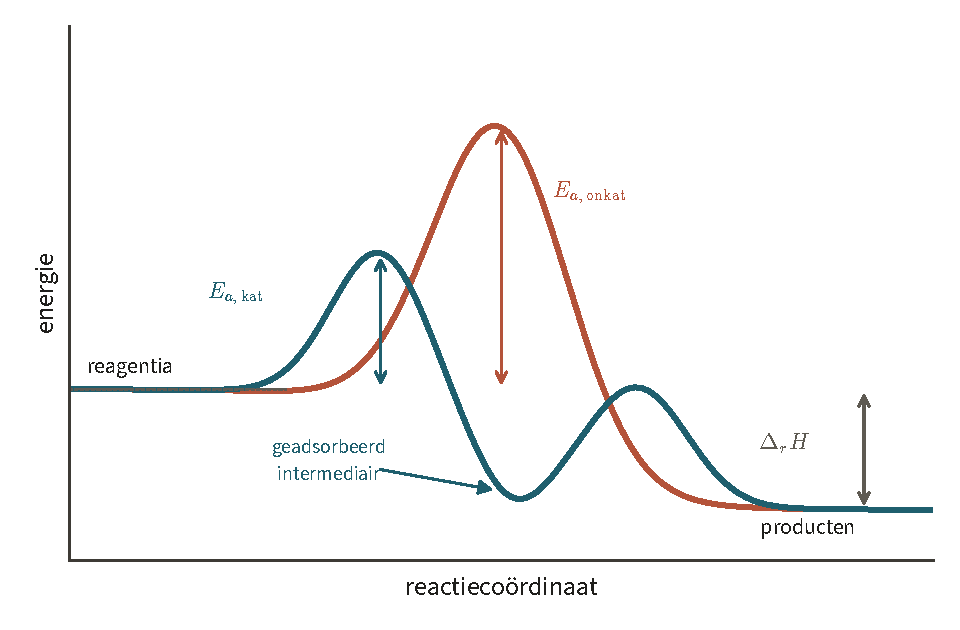
\includegraphics[width=0.7\linewidth]{Figuren/reactiecoordinaat}
    \caption{Energieprofiel met en zonder katalysator. De katalysator biedt een andere weg met lagere barri\`eres, vaak via een geadsorbeerd intermediair. Begin- en eindtoestand blijven dezelfde: $\Delta_rH$ en de evenwichtsligging veranderen niet.}
    \label{fig:reactiecoordinaat-katalysator}
\end{figure}

\subsection{Homogeen versus heterogeen}
\label{sec:homogeen-heterogeen}

Het belangrijkste onderscheid voor de ingenieur is de fase (tabel~\ref{tab:homogeen-heterogeen}). Homogene katalysatoren zijn vaak selectiever en via hun liganden fijn af te stemmen, maar het product moet er nadien van gescheiden worden. Een vast katalysatorbed scheidt zichzelf. Daarom zijn de grote processen (Haber--Bosch, het contactproces, katalytisch kraken) bijna allemaal heterogeen.

\begin{table}[htb]
\centering
\caption{Homogene en heterogene katalyse vergeleken.}
\label{tab:homogeen-heterogeen}
\begin{tabular}{lll}
\toprule
 & Homogeen & Heterogeen \\
\midrule
Fase katalysator & zelfde fase als reactanten & andere fase (meestal vast) \\
Actieve plaatsen & elke molecule & enkel oppervlakteatomen \\
Selectiviteit & doorgaans hoog, afstembaar & vaak lager, wel robuust \\
Productscheiding & moeilijk (destillatie) & eenvoudig (vast bed) \\
Thermische stabiliteit & beperkt & doorgaans hoog \\
Voorbeelden & zuur/base, Rh-complex, enzym & Fe, \ce{V2O5}, Pt, zeoliet \\
\bottomrule
\end{tabular}
\end{table}

\subsection{Homogene katalyse}
\label{sec:homogene-katalyse}

Typische homogene katalysatoren zijn zuren en basen (esterhydrolyse, inversie van sucrose), opgeloste metaalcomplexen (de Wilkinsonkatalysator \ce{RhCl(PPh3)3} voor hydrogenering, Pd voor koppelingsreacties) en enzymen. Het \emph{Monsanto-proces} zet methanol en CO om tot azijnzuur met een opgelost rhodiumcomplex bij \SIrange{150}{200}{\celsius} en \SIrange{30}{60}{\bar}, met een selectiviteit boven \SI{99}{\percent}.

\subsection{Heterogene katalyse}
\label{sec:heterogene-katalyse}

Een reactie op een vaste katalysator doorloopt vijf stappen (figuur~\ref{fig:katalyse-stappen}): (1) diffusie naar het oppervlak, (2) adsorptie, (3) reactie aan het oppervlak, (4) desorptie, (5) diffusie terug naar de gasfase. De traagste stap bepaalt de snelheid.

\begin{figure}[htb]
    \centering
    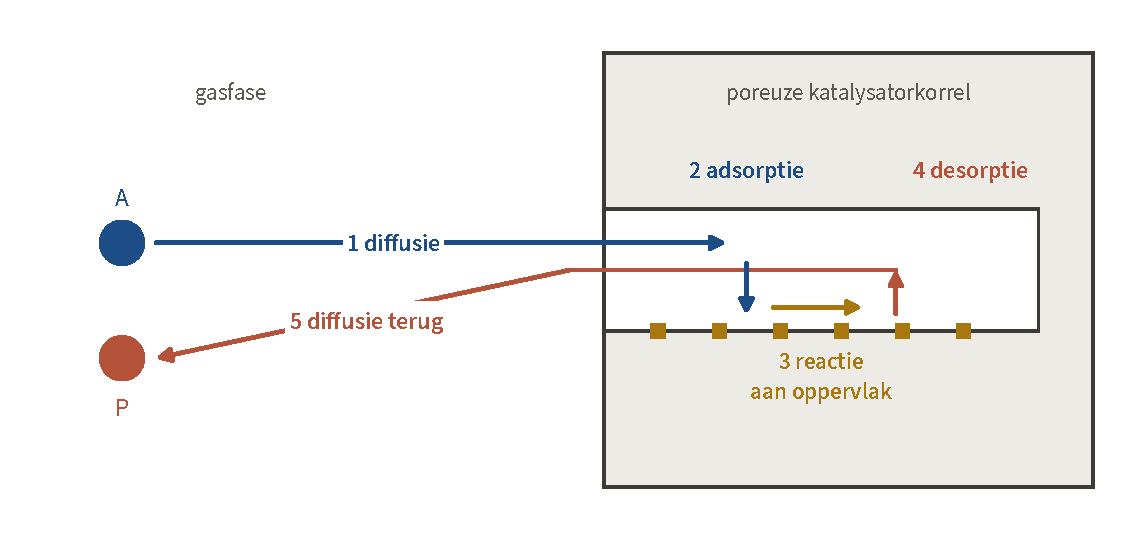
\includegraphics[width=0.85\linewidth]{Figuren/katalyse_stappen}
    \caption{De vijf stappen van een heterogeen gekatalyseerde reactie in een poreuze katalysatorkorrel. Stappen 1 en 5 zijn transport, stappen 2 tot 4 oppervlaktechemie.}
    \label{fig:katalyse-stappen}
\end{figure}

\subsubsection{Diffusie: stappen 1 en 5}
\label{sec:diffusie-katalyse}

Diffusie volgt de \emph{eerste wet van Fick}: de flux is evenredig met de concentratiegradi\"ent,
\begin{equation}
\boxed{\;j = -D\,\frac{\dd{c}}{\dd{x}}\;}
\label{eq:fick}
\end{equation}
met $D$ de diffusieco\"effici\"ent (\si{\metre\squared\per\second}). Daaruit volgt de belangrijkste vuistregel van transport: de tijd om een afstand $L$ te overbruggen, schaalt met het \emph{kwadraat} van die afstand,
\begin{equation}
\boxed{\;t_{\text{diff}} \approx \frac{L^2}{D}\;}
\label{eq:diffusietijdschaal}
\end{equation}

\begin{voorbeeld}{Diffusietijd in een poreuze katalysatorkorrel}
Met $D \approx \SI{1e-5}{\metre\squared\per\second}$ (gas in poriën) is $t_\text{diff} \approx \SI{0.1}{\second}$ voor een korrel met straal \SI{1}{\milli\metre}, maar slechts \SI{10}{\micro\second} voor \SI{10}{\micro\metre}. Honderd keer kleiner is tienduizend keer sneller. Kleine korrels houden de oppervlaktereactie snelheidsbepalend, maar geven een grotere drukval over het bed: een klassieke ontwerpafweging voor Reactorentechnologie.
\end{voorbeeld}

\subsubsection{Adsorptie en Langmuir--Hinshelwood-kinetiek}
\label{sec:adsorptie-kinetiek}
\label{sec:langmuir-hinshelwood}

Adsorptie (fysisorptie en chemisorptie, de Langmuir-isotherme, BET) kwam aan bod in hoofdstuk~\ref{ch:grensvlakken} (\S~\ref{sec:fysisorptie-chemisorptie} tot \S~\ref{sec:bet}). Chemisorptie verzwakt de bindingen van het reagens en verlaagt zo de barri\`ere van de oppervlaktereactie. Moeten \emph{beide} reactanten adsorberen en is de oppervlaktereactie snelheidsbepalend, dan is $r = k\,\theta_A\theta_B$. Met de competitieve Langmuir-isotherme (vergelijking~\eqref{eq:langmuir-competitief}) volgt de \emph{Langmuir--Hinshelwood}-snelheidswet:
\begin{equation}
r = \frac{k\,K_A\,K_B\,p_A\,p_B}{(1 + K_A\,p_A + K_B\,p_B)^2}.
\label{eq:langmuir-hinshelwood}
\end{equation}
Bij lage druk is het oppervlak bijna leeg en $r \approx kK_AK_Bp_Ap_B$. Bij hoge $p_A$ verdringt $A$ het andere reagens van het oppervlak, en de snelheid \emph{daalt} weer (figuur~\ref{fig:lh-vs-er}). Zo werkt CO-oxidatie op platina, en zo werkt ook de ammoniaksynthese op ijzer.

\subsubsection{Eley--Rideal-kinetiek}
\label{sec:eley-rideal}
\label{sec:lh-vs-er-onderscheid}

Bij het \emph{Eley--Rideal}-mechanisme adsorbeert enkel $A$, en $B$ reageert er rechtstreeks vanuit de gasfase mee:
\begin{equation}
r = k\,\theta_A\,p_B = \frac{k\,K_A\,p_A\,p_B}{1+K_A\,p_A}.
\label{eq:eley-rideal}
\end{equation}
Bij lage $p_A$ geven beide mechanismen hetzelfde. Bij hoge $p_A$ verschillen ze: Langmuir--Hinshelwood heeft een maximum, Eley--Rideal stijgt naar een plateau, want een volledig met $A$ bedekt oppervlak is voor $B$ juist ideaal. Dat verschil in het hogedrukgedrag is het experimentele criterium om beide te onderscheiden.

\begin{figure}[htb]
    \centering
    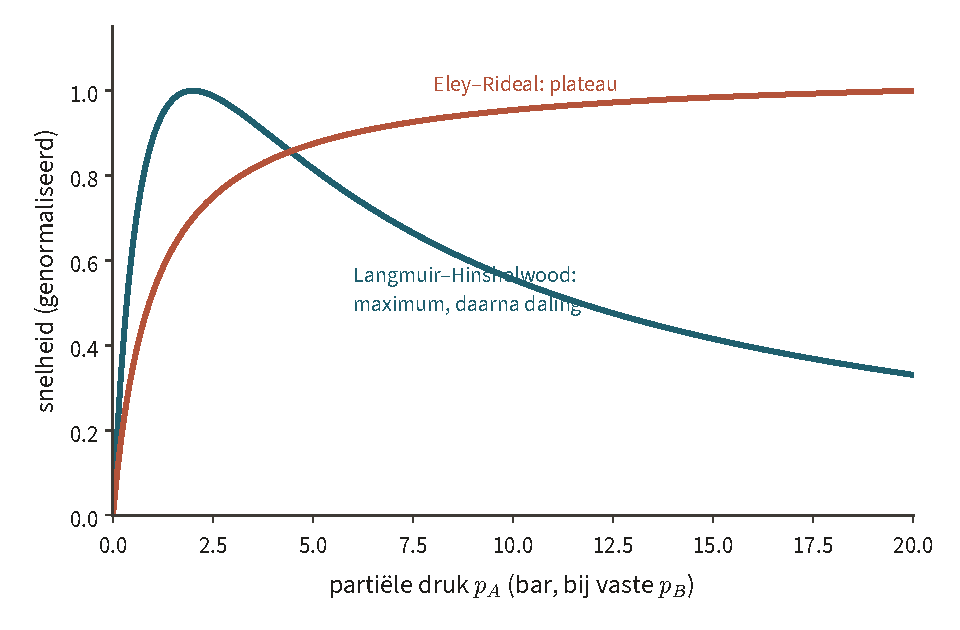
\includegraphics[width=0.7\linewidth]{Figuren/lh_er}
    \caption{Reactiesnelheid als functie van $p_A$ bij vaste $p_B$ volgens Langmuir--Hinshelwood (maximum, daarna daling door verdringing van $B$) en Eley--Rideal (monotone stijging naar een plateau).}
    \label{fig:lh-vs-er}
\end{figure}

\begin{toepassing}{Industri\"ele katalysatoren}
\begin{itemize}
\item \textbf{Haber--Bosch}: \ce{Fe3O4} met promotoren (\ce{K2O}, \ce{Al2O3}), \SIrange{400}{500}{\celsius}, \SIrange{150}{300}{\bar}. Snelheidsbepalend is de dissociatieve chemisorptie van \ce{N2}.
\item \textbf{Contactproces}: \ce{V2O5} voor \ce{SO2 -> SO3} bij \SIrange{400}{500}{\celsius}.
\item \textbf{Katalytisch kraken (FCC)}: zeolieten bij \SIrange{500}{600}{\celsius}. Thermisch kraken vroeg \SIrange{700}{800}{\celsius} en gaf veel cokes; de zeoliet verlaagt $E_a$ van meer dan \SI{250}{} tot ongeveer \SI{150}{\kilo\joule\per\mole} en is veel selectiever naar benzine.
\item \textbf{Driewegkatalysator}: Pt, Pd, Rh op \ce{Al2O3} oxideert CO en koolwaterstoffen en reduceert \ce{NO_x}, met Langmuir--Hinshelwood-kinetiek.
\item \textbf{Methanolsynthese}: \ce{Cu/ZnO/Al2O3} bij \SIrange{200}{300}{\celsius}.
\end{itemize}
\end{toepassing}

\section{Enzymkinetiek: Michaelis--Menten}
\label{sec:michaelis-menten}

Een enzym $E$ bindt zijn substraat $S$ tot een complex, dat het product vrijgeeft:
\begin{equation}
E + S \xrightleftharpoons[k_{-1}]{k_1} ES \xrightarrow{k_2} E + P.
\end{equation}
Steady state voor $ES$ en de massabalans $[E]_0 = [E] + [ES]$ geven de \emph{Michaelis--Mentenvergelijking}:
\begin{equation}
\boxed{\;r = \frac{r_{\max}\,[S]}{K_M + [S]}\;}
\qquad\text{met}\quad r_{\max} = k_2[E]_0, \quad K_M = \frac{k_{-1} + k_2}{k_1}.
\end{equation}
$K_M$ is de substraatconcentratie waarbij $r = r_{\max}/2$. Bij $[S] \ll K_M$ is de reactie eerste orde, bij $[S] \gg K_M$ nulde orde: alle enzymen zijn bezet. De vergelijking heeft exact de vorm van de Langmuir-isotherme (vergelijking~\eqref{eq:langmuir-isotherm}); in beide gevallen verzadigt een eindig aantal bindingsplaatsen. Een voorbeeld: met $K_M = \SI{2.0}{\milli\mole\per\litre}$ geeft $[S] = K_M$ de helft van $r_{\max}$, en tien keer meer substraat slechts \SI{91}{\percent} van $r_{\max}$.

\subsection{Diffusielimitatie}
\label{sec:diffusielimitatie}

Enzym en substraat moeten elkaar eerst vinden. Sneller dan diffusie toelaat, kan dat niet. Volgens Smoluchowski is de maximale bimoleculaire snelheidsconstante in oplossing
\begin{equation}
\boxed{\;k_D = 4\pi N_A\,(D_A+D_B)\,(r_A+r_B)\;}
\label{eq:smoluchowski}
\end{equation}
Voor een klein substraat ($D \approx \SI{1e-9}{\metre\squared\per\second}$, $r \approx \SI{0.5}{\nano\metre}$) en een enzym ($D \approx \SI{1e-10}{\metre\squared\per\second}$, $r \approx \SI{3}{\nano\metre}$) is $k_D \approx \SI{3e10}{\litre\per\mole\per\second}$. Enzymen die dit benaderen (carboanhydrase, triosefosfaatisomerase) heten \emph{diffusie-perfect}: elke ontmoeting leidt tot reactie.

De diffusieco\"effici\"ent van een bolvormig deeltje schat je met de \emph{vergelijking van Stokes--Einstein}:
\begin{equation}
\boxed{\;D = \frac{k_BT}{6\pi\eta r}\;}
\label{eq:stokes-einstein}
\end{equation}
Een opgeloste metaalcomplexkatalysator ($r \approx \SI{0.7}{\nano\metre}$) in tolueen ($\eta = \SI{6e-4}{\pascal\second}$) heeft $D \approx \SI{5e-10}{\metre\squared\per\second}$, vijf keer trager dan een klein substraatmolecule. In een grote reactor moet roeren, niet diffusie, de stoffen bijeenbrengen.

\section{Kinetiek en reactorontwerp}

Het vak Reactorentechnologie (Levenspiel) werkt reactorontwerp uit; hier enkel de kern. De benodigde verblijftijd $\tau$ volgt uit de snelheidswet. Voor een eerste-orde reactie met omzetting $X$:
\begin{equation}
\tau_\text{batch/PFR} = \frac{1}{k}\ln\frac{1}{1-X},
\qquad
\tau_\text{CSTR} = \frac{1}{k}\,\frac{X}{1-X}.
\end{equation}
In een ideaal geroerde tank (CSTR) heerst overal de lage eindconcentratie, in een batch- of propstroomreactor (PFR) daalt de concentratie geleidelijk. Voor $X = 0.90$ en $k = \SI{0.05}{\per\second}$ is $\tau_\text{PFR} = \SI{46}{\second}$ en $\tau_\text{CSTR} = \SI{180}{\second}$: de tank moet bijna vier keer groter zijn. Voor een tweede-orde reactie in een batchreactor is $\tau = X/(k[A]_0(1-X))$.


\section{Warmte en snelheid: wanneer een reactor op hol slaat}
\label{sec:runaway}

Een exotherme reactie warmt de reactor op, en een warmere reactor reageert sneller. Zolang de koeling de warmte afvoert, vindt de reactor een stabiel werkpunt. Lukt dat niet meer, dan versnelt de reactie zichzelf: \emph{thermische runaway}.

De warmteproductie is evenredig met de reactiesnelheid en stijgt dus exponentieel met de temperatuur:
\[
\dot Q_\mathrm{prod} = (-\Delta_rH)\,V\,k_0\,e^{-E_a/RT}\,c^n.
\]
De warmteafvoer door een koelmantel met koelmiddel op $T_c$ is lineair in $T$:
\[
\dot Q_\mathrm{afv} = UA\,(T - T_c).
\]
In een \emph{Semenovdiagram} (figuur~\ref{fig:semenov}) zie je beide curves. Waar ze snijden, is er evenwicht. Het onderste snijpunt is stabiel: wordt de reactor iets warmer, dan stijgt de afvoer sneller dan de productie en koelt hij terug af. Wordt het koelmiddel warmer of de koeling zwakker, dan schuift de rechte naar rechts tot ze de exponenti\"ele curve enkel nog raakt. Daarna is er geen snijpunt meer en loopt de temperatuur weg.

\begin{figure}[htb]
    \centering
    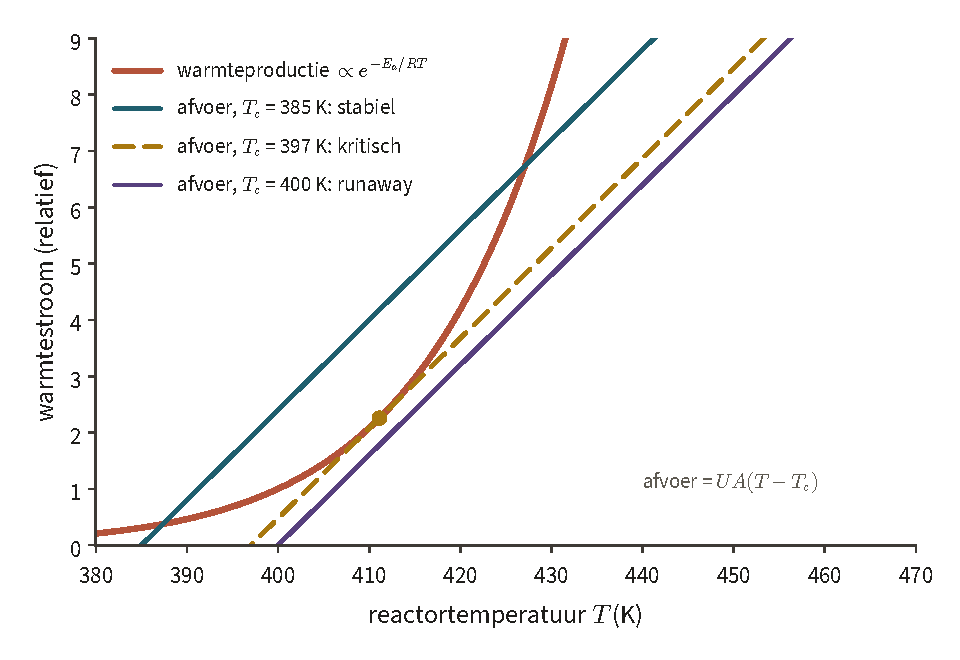
\includegraphics[width=0.7\linewidth]{Figuren/semenov}
    \caption{Semenovdiagram van een gekoelde reactor ($E_a = \SI{100}{\kilo\joule\per\mole}$, illustratieve waarden). Bij een koelmiddel van \SI{385}{\kelvin} is er een stabiel werkpunt. Bij \SI{397}{\kelvin} raakt de afvoerrechte de productiecurve: de kritische toestand. Bij \SI{400}{\kelvin} is er geen snijpunt meer: runaway.}
    \label{fig:semenov}
\end{figure}

Uit de raakvoorwaarde (gelijke waarde \'en gelijke helling) volgt een eenvoudige vuistregel: op het kritische punt ligt de reactortemperatuur ongeveer
\begin{equation}
\boxed{\;\Delta T_\mathrm{krit} \approx \frac{RT_c^2}{E_a}\;}
\label{eq:semenov}
\end{equation}
boven die van het koelmiddel. Voor $E_a = \SI{100}{\kilo\joule\per\mole}$ en $T_c = \SI{397}{\kelvin}$ is dat $8.314\cdot397^2/100\,000 = \SI{13}{\kelvin}$. Een reactor die meer dan een tiental graden warmer draait dan zijn koelmiddel, werkt dicht bij de grens. Hoe hoger $E_a$, hoe kleiner de marge.

\begin{toepassing}{Seveso en de veiligheid van chemische installaties}
Op 10 juli 1976 liep in een fabriek in Meda, bij Seveso (Itali\"e), een reactor voor trichloorfenol warm nadat de batch tijdens het weekend was stilgelegd zonder volledige afkoeling. Een exotherme nevenreactie versnelde zichzelf, de breekplaat opende en een wolk met dioxine (TCDD) kwam vrij over de omgeving. De ramp leidde tot de Europese Sevesorichtlijn, vandaag Seveso III. Bedrijven die grote hoeveelheden gevaarlijke stoffen behandelen, waaronder veel bedrijven in de haven van Antwerpen, moeten hun risico's op runaway en andere zware ongevallen analyseren en beheersen. De ingenieur gebruikt daarvoor de begrippen uit dit hoofdstuk en hoofdstuk~\ref{ch:energie}: de adiabatische temperatuurstijging (\S~\ref{sec:warmte-effecten}) zegt hoe ver de temperatuur kan oplopen, de activeringsenergie zegt hoe snel.
\end{toepassing}

\section{De brug tussen thermodynamica en kinetiek}
\label{sec:brug-thermo-kinetiek}

Voor een omkeerbare elementaire reactie $A \rightleftharpoons B$ is $K = k_1/k_{-1}$ (\S~\ref{sec:omkeerbare-reacties}). Beide constanten volgen Arrhenius, dus $\dd\ln k/\dd T = E_a/RT^2$ voor elk. Aftrekken geeft
\[
\frac{\dd{\ln K}}{\dd{T}} = \frac{E_{a,\text{heen}} - E_{a,\text{terug}}}{RT^2}.
\]
Vergelijk met Van 't Hoff (vergelijking~\eqref{eq:vanthoff-diff}), $\dd\ln K/\dd T = \Delta_rH^\circ/RT^2$:
\begin{equation}
\boxed{\;E_{a,\text{heen}} - E_{a,\text{terug}} \approx \Delta_r H^\circ\;}
\label{eq:Ea-verschil-drH}
\end{equation}
Dat zie je ook in figuur~\ref{fig:reactiecoordinaat-katalysator}: het hoogteverschil tussen begin- en eindtoestand is $\Delta_rH$, welke weg je ook neemt. Een exotherme reactie heeft dus altijd een lagere barri\`ere heen dan terug.

\subsection{Temperatuursgevoeligheid van exotherme en endotherme reacties}
\label{sec:temperatuursgevoeligheid}

Hoe groter $E_a$, hoe gevoeliger $k$ voor de temperatuur. Bij een exotherme evenwichtsreactie versnelt de \emph{terug}reactie dus sterker bij opwarming dan de heenreactie.

\begin{voorbeeld}{Ammoniaksynthese: heen- en terugreactie}
Met $E_{a,\text{heen}} \approx \SI{230}{\kilo\joule\per\mole}$ (\S~\ref{sec:ammoniak-arrhenius}) en $\Delta_rH^\circ \approx \SI{-92}{\kilo\joule\per\mole}$ is $E_{a,\text{terug}} = 230 + 92 = \SI{322}{\kilo\joule\per\mole}$. Van \SI{300}{\kelvin} naar \SI{700}{\kelvin} stijgt $k_\text{heen}$ met een factor $7.7\times10^{22}$, maar $k_\text{terug}$ met $1.1\times10^{32}$: tien grootteordes meer. Daarom daalt $K = k_\text{heen}/k_\text{terug}$ van ongeveer $6\times10^5$ naar $3\times10^{-4}$, precies wat Van 't Hoff ook gaf (\S~\ref{sec:vanthoff-reagerend}). Thermodynamica en kinetiek vertellen hetzelfde verhaal.
\end{voorbeeld}

\section{Industri\"ele toepassingen: een overzicht}

Bij elk proces zoekt de ingenieur een compromis tussen evenwicht (thermodynamica) en snelheid (kinetiek), en de katalysator verschuift dat compromis.
\begin{itemize}
\item \textbf{Haber--Bosch} en het \textbf{contactproces}: exotherm, dus lage $T$ geeft meer opbrengst, maar zonder \SIrange{400}{500}{\celsius} is de reactie te traag.
\item \textbf{Methanolsynthese}: ook exotherm, maar een actievere koperkatalysator laat \SIrange{200}{300}{\celsius} toe.
\item \textbf{Stoomreforming van methaan}: endotherm; zowel evenwicht als snelheid vragen \SIrange{800}{900}{\celsius}.
\item \textbf{Driewegkatalysator}: moet bij \SIrange{300}{800}{\celsius} meer dan \SI{95}{\percent} van CO, koolwaterstoffen en \ce{NO_x} omzetten; bij een koude start is hij nog niet actief.
\end{itemize}
Een betere katalysator laat een lagere temperatuur toe (meer opbrengst) zonder dat de reactie te traag wordt.


\section{Samenvatting en reflectie}

Met dit hoofdstuk is de cirkel rond. De thermodynamica (hoofdstukken~\ref{ch:energie} tot~\ref{ch:elektrochemie}) zegt welke toestand bereikbaar is; de kinetiek zegt hoe snel en via welke weg. Selectiviteit, katalyse en reactorveiligheid zijn telkens het resultaat van beide samen.

\begin{samenvatting}{Chemische kinetiek}
\begin{itemize}
\item Snelheidswet $r = k[A]^m[B]^n$; de orde volgt uit experiment. Ge\"integreerd: nulde orde lineair, eerste orde $\ln([A]_0/[A]) = kt$ met $t_{1/2} = \ln2/k$, tweede orde $1/[A] - 1/[A]_0 = kt$.
\item Arrhenius $k = A\,e^{-E_a/RT}$; $\ln k$ tegen $1/T$ geeft $E_a$. Botsingstheorie: $A = P\sigma\bar v_\mathrm{rel}N_A$ en $e^{-E_a/RT}$ is de fractie botsingen met genoeg energie.
\item Kinetische gastheorie: $\bar v = \sqrt{8RT/\pi M}$, vrije weglengte $\lambda = k_BT/(\sqrt2\sigma p)$ (\SI{68}{\nano\metre} voor lucht bij \SI{1}{\bar}); Graham: effusie $\propto 1/\sqrt M$.
\item Omkeerbare reacties naderen het evenwicht met tijdsconstante $1/(k_1+k_{-1})$, en $K = k_1/k_{-1}$.
\item Parallelle reacties: hoge $T$ bevoordeelt de reactie met de hoogste $E_a$. Reacties in serie: het tussenproduct heeft een optimale reactietijd.
\item Mechanismen: de steady-state-benadering en de snelheidsbepalende stap leveren de snelheidswet (ozon, Lindemann, Michaelis--Menten).
\item Een katalysator verlaagt $E_a$ in beide richtingen en verandert $K$ niet. Heterogene kinetiek bouwt op de Langmuir-isotherme (Langmuir--Hinshelwood, Eley--Rideal); transport door diffusie kan de snelheid beperken.
\item Runaway: de warmteproductie stijgt exponentieel, de afvoer lineair. Kritisch bij $T - T_c \approx RT_c^2/E_a$.
\item $E_{a,\mathrm{heen}} - E_{a,\mathrm{terug}} \approx \Delta_rH^\circ$: daarom verliest een exotherm evenwicht opbrengst bij hoge temperatuur.
\end{itemize}
\end{samenvatting}

\begin{reflectie}{Chemische kinetiek}
\begin{enumerate}
\item Waarom stijgt de reactiesnelheid veel sterker met de temperatuur dan de gemiddelde snelheid van de moleculen?
\item Waarom is de halfwaardetijd van een eerste-orde reactie onafhankelijk van de beginconcentratie, en die van een tweede-orde reactie niet?
\item Een katalysator versnelt de heenreactie met een factor duizend. Wat gebeurt er met de terugreactie, en waarom?
\item Waarom kan een hogere temperatuur de opbrengst van een tussenproduct in een serie-reactie verlagen, ook al gaat alles sneller?
\item Waarom werkt men bij ethyleenoxide niet gewoon bij een hogere temperatuur om de reactor kleiner te maken?
\item Waarom is een reactor met een reactie met hoge activeringsenergie gevoeliger voor runaway?
\item Waarom diffunderen gassen in de poriën van een katalysator anders dan in een buis van een centimeter?
\item Welke stap is snelheidsbepalend in een katalytische uitlaat net na een koude start, en welke als de motor warm is?
\end{enumerate}
\end{reflectie}

\newpage
\section{Oefeningen}

% Oefeningen bij dit hoofdstuk (ingevoegd achteraan het hoofdstuk met \input).
% Een oefening:  \begin{oefening}[titel] ... \end{oefening}   (boek en website)
% De oplossing:  \begin{oplossing} ... \end{oplossing}       (enkel website, dichtgeklapt)

Neem $g = \SI{9.81}{\metre\per\second\squared}$, $\sigma_{\text{water}} = \SI{72}{\milli\newton\per\metre}$ bij \SI{20}{\celsius}, $k_B = \SI{1.381e-23}{\joule\per\kelvin}$ en $R = \SI{8.314}{\joule\per\mole\per\kelvin}$.

\begin{oefening}[Hoeveel energie kost een wolk mist?]
Een ultrasone luchtbevochtiger vernevelt water tot fijne druppeltjes zonder het te verwarmen.

\begin{enumerate}
\item[(a)]
  Toon aan dat het totale oppervlak van een volume \(V\) verdeeld in bolletjes met straal \(r\) gelijk is aan \(A = 3V/r\).
\item[(b)]
  Bereken de minimale arbeid (de toename van de Gibbs-energie) om \(1.0\,\mathrm{L}\) water te vernevelen tot druppels met \(r = 1\,\mathrm{\mu m}\) en met \(r = 10\,\mathrm{\mu m}\).
\item[(c)]
  Vergelijk met de energie om \(1.0\,\mathrm{L}\) water \(5\,^\circ\mathrm{C}\) op te warmen en om het volledig te verdampen (\(\Delta_{\text{vap}}H \approx 2.45\,\mathrm{MJ/kg}\)). Waarom is een ultrasone bevochtiger zo zuinig?
\item[(d)]
  Waarom vloeien de druppels spontaan weer samen tot grotere druppels?
\end{enumerate}
\end{oefening}
\begin{oplossing}
\textbf{Resultaat:} (b) \textbf{216 J} voor \(1\,\mathrm{\mu m}\) en \textbf{22 J} voor \(10\,\mathrm{\mu m}\). (c) Opwarmen kost \(21\,\mathrm{kJ}\), verdampen \textbf{2.45 MJ}: vernevelen vraagt ruim tienduizend keer minder energie dan verdampen. (d) Samenvloeien verkleint het oppervlak en verlaagt dus \(G\).

\textbf{(a)} Het aantal druppels is \(N = V/(\tfrac{4}{3}\pi r^3)\), elk met oppervlak \(4\pi r^2\). Dus \(A = N\cdot 4\pi r^2 = 3V/r\). Hoe kleiner de druppels, hoe groter het oppervlak.

\textbf{(b)} Met vergelijking (9.1) is \(\Delta G = \sigma\,\Delta A\) (het oorspronkelijke oppervlak is verwaarloosbaar):

\begin{itemize}
\item
  \(r = 1\,\mathrm{\mu m}\): \(A = 3\times10^{-3}/10^{-6} = 3000\,\mathrm{m^2}\), \(\Delta G = 0.072 \times 3000 = 216\,\mathrm{J}\).
\item
  \(r = 10\,\mathrm{\mu m}\): \(A = 300\,\mathrm{m^2}\), \(\Delta G = 22\,\mathrm{J}\).
\end{itemize}

Eén liter water krijgt dus het oppervlak van een half voetbalveld.

\textbf{(c)} Opwarmen: \(Q = (1\,\mathrm{kg})(4184\,\mathrm{J/(kg\cdot K)})(5\,\mathrm{K}) = 21\,\mathrm{kJ}\). Verdampen: \(2.45\,\mathrm{MJ}\). Een verdampingsbevochtiger moet de volledige verdampingsenthalpie leveren (hoofdstuk 5), een ultrasone bevochtiger enkel de oppervlakte-energie en de verliezen in de piëzokristal. Het water verdampt later in de kamer met warmte uit de omgeving, zodat de lucht wat afkoelt.

\textbf{(d)} Bij samenvloeien daalt \(A\) en dus \(G = G_{\text{bulk}} + \sigma A\): het proces is spontaan. Fijne mist is enkel kinetisch stabiel, zolang de druppels elkaar weinig raken.
\end{oplossing}

\begin{oefening}[Capillariteit: van keukenpapier tot boomtoppen]
Gebruik de wet van Jurin (9.4).

\begin{enumerate}
\item[(a)]
  Hoe hoog stijgt water (\(\rho = 1000\,\mathrm{kg/m^3}\), \(\theta = 0^\circ\)) in een glazen capillair met een binnendiameter van \(0.20\,\mathrm{mm}\)?
\item[(b)]
  Herhaal voor kwik (\(\sigma = 485\,\mathrm{mN/m}\), \(\rho = 13600\,\mathrm{kg/m^3}\), \(\theta = 140^\circ\)) in hetzelfde capillair. Verklaar het teken.
\item[(c)]
  De vezels van keukenpapier vormen poriën met een straal van ongeveer \(25\,\mathrm{\mu m}\) en een contacthoek van \(30^\circ\). Hoe hoog kan water opstijgen in een verticaal opgehangen vel?
\item[(d)]
  De houtvaten (xyleem) van een boom hebben een straal van ongeveer \(20\,\mathrm{\mu m}\). Hoe hoog brengt capillariteit het water? Welke straal zou nodig zijn voor een sequoia van \(100\,\mathrm{m}\)? Wat besluit je?
\end{enumerate}
\end{oefening}
\begin{oplossing}
\textbf{Resultaat:} (a) \textbf{14.7 cm}. (b) \textbf{\ensuremath{-}5.6 cm}: kwik daalt. (c) Ongeveer \textbf{51 cm}. (d) Slechts \textbf{0.73 m}; voor \(100\,\mathrm{m}\) zou \(r = 0.15\,\mathrm{\mu m}\) nodig zijn: capillariteit alleen verklaart het watertransport in bomen niet.

\textbf{(a)} \(h = \dfrac{2\sigma\cos\theta}{\rho g r} = \dfrac{2(0.072)(1)}{(1000)(9.81)(1.0\times10^{-4})} = 0.147\,\mathrm{m}\).

\textbf{(b)} \(h = \dfrac{2(0.485)\cos 140^\circ}{(13600)(9.81)(1.0\times10^{-4})} = -0.056\,\mathrm{m}\). Omdat \(\cos 140^\circ < 0\), is de meniscus bol en wordt het kwik naar beneden gedrukt. Kwik bevochtigt glas niet: de cohesie tussen kwikatomen (metaalbinding, hoofdstuk 2) is veel sterker dan de adhesie aan glas. Daarom lees je een kwikthermometer af aan de top van een bolle meniscus.

\textbf{(c)} \(h = \dfrac{2(0.072)\cos 30^\circ}{(1000)(9.81)(25\times10^{-6})} = 0.51\,\mathrm{m}\). Het papier zuigt een plas dus gemakkelijk op, ook tegen de zwaartekracht in. Kleinere poriën zuigen hoger, maar de stroming wordt trager.

\textbf{(d)} \(h = 0.147 \times (100/20) = 0.73\,\mathrm{m}\). Voor \(h = 100\,\mathrm{m}\): \(r = 2\sigma/(\rho g h) = 1.5\times10^{-7}\,\mathrm{m}\). In werkelijkheid trekt de verdamping uit de bladeren het water omhoog: in de minuscule poriën van de celwanden in het blad (nanometers) houdt de oppervlaktespanning een sterke negatieve druk in stand, en de waterkolom hangt dankzij de cohesie tussen watermoleculen (waterstofbruggen, hoofdstuk 4) als een touw aan die menisci.
\end{oplossing}

\begin{oefening}[Waarom bruist spuitwater aan de wand van het glas?]
In een geopende fles spuitwater is het water oververzadigd met \(\mathrm{CO_2}\): het bevat evenveel opgelost gas als in evenwicht met ongeveer \(2.5\,\mathrm{bar}\) \(\mathrm{CO_2}\) (wet van Henry, hoofdstuk 5).

\begin{enumerate}
\item[(a)]
  Bereken met Young--Laplace de overdruk in een gasbelletje met straal \(10\,\mathrm{\mu m}\), \(1\,\mathrm{\mu m}\) en \(0.1\,\mathrm{\mu m}\).
\item[(b)]
  Een belletje kan enkel groeien als de \(\mathrm{CO_2}\)-druk erin lager is dan de evenwichtsdruk van \(2.5\,\mathrm{bar}\) die het opgeloste gas ``wil'' uitoefenen. Neem een atmosferische druk van \(1\,\mathrm{bar}\). Vanaf welke straal kan een belletje groeien?
\item[(c)]
  Waarom ontstaan bellen niet midden in het water maar op krasjes, stofvezels of een Mentos-snoepje?
\item[(d)]
  Waarom bruist een glas spuitwater sterker in een glas dat niet perfect gespoeld is?
\end{enumerate}
\end{oefening}
\begin{oplossing}
\textbf{Resultaat:} (a) \textbf{0.14}, \textbf{1.44} en \textbf{14.4 bar}. (b) Groei vanaf ongeveer \textbf{\(r \approx 1\,\mathrm{\mu m}\)}. (c) Krasjes en vezels bevatten al \textbf{gaszakjes} die groter zijn dan die kritische straal. (d) Vuil en vezels leveren zulke kiemen.

\textbf{(a)} \(\Delta p = 2\sigma/r\):

\begin{itemize}
\item
  \(r = 10\,\mathrm{\mu m}\): \(\Delta p = 2(0.072)/10^{-5} = 1.44\times10^{4}\,\mathrm{Pa} = 0.14\,\mathrm{bar}\)
\item
  \(r = 1\,\mathrm{\mu m}\): \(1.44\,\mathrm{bar}\)
\item
  \(r = 0.1\,\mathrm{\mu m}\): \(14.4\,\mathrm{bar}\)
\end{itemize}

\textbf{(b)} De druk in de bel is \(p_{\text{atm}} + 2\sigma/r\). Ze kan groeien zolang die druk kleiner is dan \(2.5\,\mathrm{bar}\), dus \(2\sigma/r < 1.5\,\mathrm{bar}\), of \(r > 2(0.072)/(1.5\times10^{5}) = 0.96\,\mathrm{\mu m}\). Een kleiner belletje heeft zo'n hoge inwendige druk dat het gas er volgens Henry terug uit oplost.

\textbf{(c)} Een belletje moet spontaan uit één molecule \(\mathrm{CO_2}\) groeien tot een micrometer: alle tussenstadia zijn onstabiel, dus dat gebeurt praktisch nooit. Een kras, een vezel of het ruwe oppervlak van een Mentos houdt echter kleine luchtzakjes vast die al groter zijn dan de kritische straal. Van daaruit groeien de bellen, laten ze los en blijft er een nieuw zakje achter: zo ontstaan de bekende parelsnoeren.

\textbf{(d)} Een perfect gladde, schone glazen wand heeft weinig kiemplaatsen. Restjes vaatdoek, stof of droogvlekken zijn ideale nucleatiekiemen. Champagneglazen worden daarom soms bewust met een laser op de bodem geëtst.
\end{oplossing}

\begin{oefening}[Twee zeepbellen: welke wint?]
Twee zeepbellen met straal \(1.0\,\mathrm{cm}\) en \(3.0\,\mathrm{cm}\) (\(\sigma = 25\,\mathrm{mN/m}\)) worden via een buisje met een kraantje met elkaar verbonden.

\begin{enumerate}
\item[(a)]
  Bereken de overdruk in elke bel. Waarom staat er \(4\sigma/r\) en niet \(2\sigma/r\)?
\item[(b)]
  Wat gebeurt er wanneer het kraantje opengaat? Waar stopt het proces?
\item[(c)]
  Verklaar met hetzelfde principe waarom ijskristallen in roomijs dat lang in de diepvries ligt groter en korreliger worden, en waarom schuim op bier na een tijdje uit minder, maar grotere bellen bestaat.
\end{enumerate}
\end{oefening}
\begin{oplossing}
\textbf{Resultaat:} (a) \textbf{10 Pa} in de kleine en \textbf{3.3 Pa} in de grote bel. (b) De \textbf{kleine bel loopt leeg} in de grote, tot er enkel een gebogen filmpje met de straal van de grote bel overblijft. (c) \textbf{Ostwald-rijping}: kleine deeltjes hebben een hogere druk of chemische potentiaal en verdwijnen ten voordele van grote.

\textbf{(a)} Een zeepbel heeft twee grensvlakken (binnen- en buitenkant van de film), zodat \(\Delta p = 4\sigma/r\):

\begin{itemize}
\item
  \(r = 1.0\,\mathrm{cm}\): \(\Delta p = 4(0.025)/0.010 = 10\,\mathrm{Pa}\)
\item
  \(r = 3.0\,\mathrm{cm}\): \(\Delta p = 3.3\,\mathrm{Pa}\)
\end{itemize}

\textbf{(b)} Gas stroomt van hoge naar lage druk: de kleine bel loopt leeg in de grote. Daardoor wordt de kleine bel nog kleiner, haar druk stijgt nog meer, en het proces versnelt. Het stopt pas wanneer van de kleine bel een kapje over is met dezelfde kromtestraal als de grote bel. Dit is tegenintuïtief (je zou verwachten dat de drukken gelijk worden bij gelijke bellen), maar volgt rechtstreeks uit Young--Laplace en uit de daling van het totale oppervlak, dus van \(G\).

\textbf{(c)} Kleine ijskristallen en kleine gasbellen hebben een sterkere kromming en dus een hogere chemische potentiaal (vergelijk met de hogere druk in de bel). Watermoleculen gaan van kleine naar grote kristallen, gas diffundeert van kleine naar grote bellen. Het totale grensvlak en dus \(G\) dalen. Ijsfabrikanten voegen stabilisatoren toe en raden aan de diepvries niet te vaak te openen: elke temperatuurschommeling versnelt de rijping.
\end{oplossing}

\begin{oefening}[Wast warm water beter? Oppervlaktespanning en temperatuur]
Voor water geldt \(\sigma = 72.75\,\mathrm{mN/m}\) bij \(20\,^\circ\mathrm{C}\), met \(V_m = 18.05\,\mathrm{cm^3/mol}\) en \(T_c = 647.1\,\mathrm{K}\).

\begin{enumerate}
\item[(a)]
  Bereken de constante \(k\) in de vergelijking van Eötvös (9.2) uit deze gegevens.
\item[(b)]
  Voorspel \(\sigma\) bij \(60\,^\circ\mathrm{C}\) (\(V_m = 18.32\,\mathrm{cm^3/mol}\)) en bij \(80\,^\circ\mathrm{C}\) (\(V_m = 18.54\,\mathrm{cm^3/mol}\)). De gemeten waarden zijn \(66.2\) en \(62.6\,\mathrm{mN/m}\). Hoe goed is de voorspelling?
\item[(c)]
  Waarom daalt de oppervlaktespanning met de temperatuur, en wat gebeurt er bij het kritische punt?
\item[(d)]
  Geef twee redenen waarom een afwas in warm water beter lukt dan in koud water.
\end{enumerate}
\end{oefening}
\begin{oplossing}
\textbf{Resultaat:} (a) \(k = 1.41\times10^{-7}\,\mathrm{J/(K\cdot mol^{2/3})}\). (b) Voorspeld \textbf{63.9} en \textbf{59.3 mN/m}: ongeveer \textbf{4--5 \% te laag}. (c) Zwakkere cohesie ten opzichte van de thermische energie; \(\sigma \to 0\) bij \(T_c\). (d) Lagere \(\sigma\) en vet dat smelt en sneller oplost.

\textbf{(a)} \(k = \dfrac{\sigma V_m^{2/3}}{T_c - T} = \dfrac{(0.07275)(18.05\times10^{-6})^{2/3}}{647.1 - 293.15} = 1.41\times10^{-7}\,\mathrm{J/(K\cdot mol^{2/3})}\), dicht bij de ``universele'' waarde van ongeveer \(2.1\times10^{-7}\) voor niet-geassocieerde vloeistoffen. Water wijkt af door de waterstofbruggen.

\textbf{(b)} \(\sigma = k(T_c - T)/V_m^{2/3}\):

\begin{itemize}
\item
  \(60\,^\circ\mathrm{C}\): \(\sigma = 63.9\,\mathrm{mN/m}\) (gemeten \(66.2\), afwijking \(-3.5\,\%\))
\item
  \(80\,^\circ\mathrm{C}\): \(\sigma = 59.3\,\mathrm{mN/m}\) (gemeten \(62.6\), afwijking \(-5\,\%\))
\end{itemize}

Een empirische correlatie met één constante, gefit op één punt, extrapoleert dus redelijk maar niet perfect. Daarom gebruikt men in de praktijk varianten met een gecorrigeerde \(T_c\) (bijvoorbeeld \(T_c - 6\,\mathrm{K}\)).

\textbf{(c)} Bij hogere temperatuur is de thermische energie groter ten opzichte van de intermoleculaire aantrekking (hoofdstuk 4); het kost minder Gibbs-energie om een molecule naar het oppervlak te brengen. Bij \(T_c\) verdwijnt het onderscheid tussen vloeistof en damp (hoofdstuk 5), er is geen grensvlak meer en \(\sigma = 0\).

\textbf{(d)} Water met een lagere oppervlaktespanning bevochtigt borden en vezels beter en dringt dieper in kleine spleten. Daarnaast smelten vetten met een smeltpunt boven kamertemperatuur, verlopen oplos- en diffusieprocessen sneller (Stokes--Einstein: \(D \propto T/\eta\), en \(\eta\) daalt sterk), en werkt het afwasmiddel sneller. Het afwasmiddel zelf verlaagt \(\sigma\) nog veel meer dan de temperatuur.
\end{oplossing}

\begin{oefening}[Hoeveel afwasmiddel heb je nodig? CMC en micellen]
Natriumdodecylsulfaat (SDS, \(M = 288.4\,\mathrm{g/mol}\)) heeft een CMC van \(8.2\times10^{-3}\,\mathrm{mol/L}\) bij \(25\,^\circ\mathrm{C}\) en vormt micellen van gemiddeld \(62\) moleculen.

\begin{enumerate}
\item[(a)]
  Hoeveel gram SDS moet je minstens in een afwasbak van \(15\,\mathrm{L}\) doen om de CMC te bereiken? Moderne vaatwasmiddelen bevatten vooral niet-ionische surfactanten met een CMC rond \(1\times10^{-4}\,\mathrm{mol/L}\) (\(M \approx 530\,\mathrm{g/mol}\)). Hoeveel gram is dan nodig?
\item[(b)]
  Een oplossing bevat \(1.0\times10^{-2}\,\mathrm{mol/L}\) SDS. Hoeveel SDS is vrij opgelost, en hoeveel micellen zijn er per liter?
\item[(c)]
  In een eenvoudig model geldt \(\Delta G^\circ_{\text{mic}} \approx RT\ln x_{\text{CMC}}\), met \(x_{\text{CMC}}\) de molfractie surfactant bij de CMC. Bereken \(\Delta G^\circ_{\text{mic}}\) per mol surfactant. Met \(\Delta H^\circ_{\text{mic}} \approx -1.5\,\mathrm{kJ/mol}\): bereken \(T\Delta S^\circ_{\text{mic}}\). Wat is de drijvende kracht?
\item[(d)]
  Waarom wordt een afwasmiddel minder doeltreffend in een gootsteen vol vet?
\end{enumerate}
\end{oefening}
\begin{oplossing}
\textbf{Resultaat:} (a) \textbf{35 g} SDS, maar slechts ongeveer \textbf{0.8 g} niet-ionische surfactant. (b) Vrij: \textbf{\(8.2\times10^{-3}\,\mathrm{mol/L}\)}; micellen: \textbf{\(2.9\times10^{-5}\,\mathrm{mol/L}\)} (\(1.7\times10^{19}\) per liter). (c) \(\Delta G^\circ_{\text{mic}} \approx\) \textbf{\ensuremath{-}21.9 kJ/mol} en \(T\Delta S^\circ \approx\) \textbf{+20 kJ/mol}: entropisch gedreven. (d) Het vet verbruikt de surfactant tot de vrije concentratie onder de CMC zakt.

\textbf{(a)} SDS: \(15\,\mathrm{L} \times 8.2\times10^{-3}\,\mathrm{mol/L} \times 288.4\,\mathrm{g/mol} = 35\,\mathrm{g}\), een flinke scheut. Niet-ionisch: \(15 \times 1\times10^{-4} \times 530 = 0.8\,\mathrm{g}\). Een lagere CMC betekent dat veel minder product nodig is om micellen te vormen; daarom zijn moderne, geconcentreerde wasmiddelen zo zuinig. Een lange hydrofobe staart en het ontbreken van een geladen kop (geen elektrostatische afstoting tussen de koppen) verlagen de CMC.

\textbf{(b)} Boven de CMC blijft de vrije concentratie gelijk aan de CMC: \(8.2\times10^{-3}\,\mathrm{mol/L}\). De rest, \(1.8\times10^{-3}\,\mathrm{mol/L}\), zit in micellen: \(1.8\times10^{-3}/62 = 2.9\times10^{-5}\,\mathrm{mol/L}\) micellen, of \(1.7\times10^{19}\) micellen per liter.

\textbf{(c)} Met \(55.5\,\mathrm{mol/L}\) water: \(x_{\text{CMC}} = 8.2\times10^{-3}/55.5 = 1.48\times10^{-4}\), dus \(\Delta G^\circ_{\text{mic}} = (8.314)(298.15)\ln(1.48\times10^{-4}) = -21.9\,\mathrm{kJ/mol}\). Dan \(T\Delta S^\circ = \Delta H^\circ - \Delta G^\circ = -1.5 + 21.9 = +20.4\,\mathrm{kJ/mol}\). Bijna de volledige drijvende kracht is entropisch: het hydrofoob effect (§9.4.2). De geordende watermoleculen rond de koolwaterstofstaarten komen vrij wanneer de staarten in de micel verdwijnen (hoofdstuk 3, \(\Delta G = \Delta H - T\Delta S\)).

\textbf{(d)} Vet wordt opgelost in de kern van de micellen en surfactant adsorbeert aan het grote vet--watergrensvlak. Dat onttrekt surfactant aan de oplossing. Zakt de vrije concentratie onder de CMC, dan verdwijnen de micellen, stijgt de oppervlaktespanning en komt het vet terug vrij. Bij een zeer vette afwas moet je dus water verversen of meer middel toevoegen.
\end{oplossing}

\begin{oefening}[De zeta-potentiaal van klei meten met elektroforese]
Kleideeltjes in rivierwater bewegen in een elektrisch veld van \(1000\,\mathrm{V/m}\) met een snelheid van \(35\,\mathrm{\mu m/s}\) naar de positieve elektrode. Na toevoegen van \(10\,\mathrm{mmol/L}\) \(\mathrm{CaCl_2}\) daalt de snelheid tot \(9.5\,\mathrm{\mu m/s}\). Volgens de vergelijking van Smoluchowski is de elektroforetische mobiliteit \(u = v/E = \varepsilon_r\varepsilon_0\zeta/\eta\), met voor water \(\varepsilon_r = 78.5\), \(\varepsilon_0 = 8.854\times10^{-12}\,\mathrm{F/m}\) en \(\eta = 8.9\times10^{-4}\,\mathrm{Pa\,s}\).

\begin{enumerate}
\item[(a)]
  Wat is het teken van de oppervlaktelading van de kleideeltjes?
\item[(b)]
  Bereken de zeta-potentiaal voor en na toevoegen van \(\mathrm{CaCl_2}\).
\item[(c)]
  Voorspel de stabiliteit van de dispersie in beide gevallen.
\item[(d)]
  Waarom is \(\mathrm{Ca^{2+}}\) veel doeltreffender dan \(\mathrm{Na^+}\), en waarom gebruiken drinkwaterbedrijven \(\mathrm{Al^{3+}}\)-zouten?
\item[(e)]
  Waarom is het water aan de monding van een rivier in de zee vaak troebel en slibt de haven er dicht?
\end{enumerate}
\end{oefening}
\begin{oplossing}
\textbf{Resultaat:} (a) \textbf{Negatief}. (b) \(\zeta \approx\) \textbf{\ensuremath{-}45 mV} voor en \textbf{\ensuremath{-}12 mV} na toevoegen. (c) Eerst \textbf{stabiel} (\(|\zeta| > 30\,\mathrm{mV}\)), daarna bijna aan de grens van \textbf{snelle coagulatie}. (d) Meerwaardige tegenionen comprimeren de dubbellaag veel sterker. (e) Zeewater is een zoutoplossing: de klei coaguleert en bezinkt.

\textbf{(a)} De deeltjes bewegen naar de positieve elektrode: ze zijn negatief geladen. Klei krijgt die lading door isomorfe substitutie (\(\mathrm{Al^{3+}}\) in plaats van \(\mathrm{Si^{4+}}\) in het kristalrooster) en door ionisatie van randgroepen.

\textbf{(b)} \(\zeta = \dfrac{u\,\eta}{\varepsilon_r\varepsilon_0}\) met \(\varepsilon_r\varepsilon_0 = 6.95\times10^{-10}\,\mathrm{F/m}\):

\begin{itemize}
\item
  voor: \(u = 3.5\times10^{-8}\,\mathrm{m^2/(V\cdot s)}\), \(\zeta = \dfrac{(3.5\times10^{-8})(8.9\times10^{-4})}{6.95\times10^{-10}} = 0.045\,\mathrm{V}\), dus \(\zeta = -45\,\mathrm{mV}\)
\item
  na: \(u = 9.5\times10^{-9}\,\mathrm{m^2/(V\cdot s)}\), \(\zeta = -12\,\mathrm{mV}\)
\end{itemize}

\textbf{(c)} Met \(|\zeta| = 45\,\mathrm{mV}\) is er een hoge DLVO-energiedrempel en blijft de klei zweven: het water blijft troebel. Bij \(12\,\mathrm{mV}\) is de afstoting bijna verdwenen en domineert de Van der Waals-aantrekking: de deeltjes klonteren samen tot vlokken die bezinken.

\textbf{(d)} Een tegenion met een hogere lading schermt de oppervlaktelading veel efficiënter af: de dubbellaag wordt dunner (kleinere Debye-lengte) en \(\zeta\) daalt, en tweewaardige ionen worden bovendien sterker in de Stern-laag gebonden. Empirisch neemt de benodigde coagulatieconcentratie zeer sterk af met de lading van het tegenion (de regel van Schulze--Hardy): \(\mathrm{Al^{3+}}\) werkt al bij veel lagere doses dan \(\mathrm{Ca^{2+}}\), en die op hun beurt veel beter dan \(\mathrm{Na^+}\). Bovendien vormt \(\mathrm{Al^{3+}}\) in water vlokkig \(\mathrm{Al(OH)_3}\) dat de deeltjes mee insluit.

\textbf{(e)} Zeewater bevat ongeveer \(0.5\,\mathrm{mol/L}\) \(\mathrm{NaCl}\) en daarnaast \(\mathrm{Mg^{2+}}\) en \(\mathrm{Ca^{2+}}\). Waar rivierwater zich met zeewater mengt, coaguleert de klei en bezinkt ze. Zo ontstaan slikken en schorren, en moet een haven als Antwerpen of Zeebrugge voortdurend gebaggerd worden.
\end{oplossing}

\begin{oefening}[Mayonaise en dressing: grensvlak en HLB]
Mayonaise bevat ongeveer \(80\,\mathrm{vol\%}\) olie in de vorm van druppels met een straal van ongeveer \(1\,\mathrm{\mu m}\) in een waterfase met eigeel en azijn.

\begin{enumerate}
\item[(a)]
  Bereken het olie--watergrensvlak in \(1\,\mathrm{L}\) mayonaise.
\item[(b)]
  Bereken de grensvlakenergie bij een grensvlakspanning van \(30\,\mathrm{mN/m}\) (zonder emulgator) en \(5\,\mathrm{mN/m}\) (met eigeel). Is mayonaise thermodynamisch stabiel?
\item[(c)]
  Een fabrikant wil een vinaigrette (O/W) stabiliseren met een mengsel van Span 80 (HLB \(4.3\)) en Tween 80 (HLB \(15.0\)) en mikt op een HLB van \(10\). Het HLB-getal van een mengsel is het massagewogen gemiddelde. Welk massapercentage Tween 80 is nodig?
\item[(d)]
  Welke emulgator (Span 80 alleen of Tween 80 alleen) kies je voor een W/O-product zoals een vette handcrème of margarine? Verklaar met de structuur van de moleculen.
\end{enumerate}
\end{oefening}
\begin{oplossing}
\textbf{Resultaat:} (a) \textbf{2400 m\ensuremath{^{2}}} per liter. (b) \textbf{72 J} zonder en \textbf{12 J} met emulgator; mayonaise blijft \textbf{thermodynamisch onstabiel}, maar is kinetisch stabiel. (c) Ongeveer \textbf{53 \%} Tween 80. (d) \textbf{Span 80} (HLB 4.3).

\textbf{(a)} Met \(A = 3V_{\text{olie}}/r\) (oefening 9.1): \(A = 3(0.80\times10^{-3}\,\mathrm{m^3})/(1\times10^{-6}\,\mathrm{m}) = 2400\,\mathrm{m^2}\).

\textbf{(b)} \(G_{\text{grensvlak}} = \sigma A\): \(0.030 \times 2400 = 72\,\mathrm{J}\) zonder emulgator, \(0.005 \times 2400 = 12\,\mathrm{J}\) met eigeel. Ook met emulgator blijft \(\Delta G > 0\) ten opzichte van een gescheiden laag olie en water: de emulsie is thermodynamisch onstabiel (§9.6). Lecithine en eiwitten uit het eigeel verlagen de energie die je met de garde moet leveren en vormen vooral een beschermende laag die het samenvloeien van druppels kinetisch verhindert. Bij te veel opwarmen of invriezen breekt die laag en ``schift'' de mayonaise.

\textbf{(c)} Met \(w\) de massafractie Tween 80: \(15.0\,w + 4.3(1 - w) = 10\), dus \(w = 5.7/10.7 = 0.53\), of \(53\,\%\) Tween 80 en \(47\,\%\) Span 80. Mengsels van een hydrofiele en een lipofiele emulgator laten toe het HLB-getal fijn af te stemmen.

\textbf{(d)} Voor een W/O-emulsie is een lipofiele emulgator met HLB \(3\)--\(6\) nodig: Span 80 (sorbitanmono-oleaat) heeft een kleine polaire kop en een lange oliezuurstaart, en buigt het grensvlak rond de waterdruppels. Tween 80 is hetzelfde molecule met lange polyethyleenoxideketens aan de kop: sterk hydrofiel, en dus geschikt voor O/W (melk, dressing, vloeibare geneesmiddelen).
\end{oplossing}

\begin{oefening}[Waarom roomt gehomogeniseerde melk niet op?]
Vetbolletjes in rauwe melk hebben een straal van ongeveer \(1.5\,\mathrm{\mu m}\); na homogeniseren is dat ongeveer \(0.25\,\mathrm{\mu m}\). De dichtheid van melkvet is \(920\,\mathrm{kg/m^3}\), die van de waterfase \(1030\,\mathrm{kg/m^3}\), en de viscositeit van de waterfase \(2.0\times10^{-3}\,\mathrm{Pa\,s}\). De snelheid waarmee een bolletje opstijgt is gegeven door de wet van Stokes, \(v = 2r^2\Delta\rho\,g/(9\eta)\).

\begin{enumerate}
\item[(a)]
  Bereken de opstijgsnelheid (in cm per dag) voor beide groottes.
\item[(b)]
  Bereken met Stokes--Einstein (hoofdstuk 8, vergelijking (8.35)) de diffusiecoëfficiënt bij \(20\,^\circ\mathrm{C}\), en de typische afstand die een bolletje door Brownse beweging aflegt in één dag (\(\sqrt{2Dt}\)).
\item[(c)]
  Verklaar waarom op rauwe melk na een dag een roomlaag ligt, maar niet op gehomogeniseerde melk.
\item[(d)]
  Waarom vallen deeltjes kleiner dan \(1\,\mathrm{\mu m}\) onder de definitie van een colloïde (§9.5)?
\end{enumerate}
\end{oefening}
\begin{oplossing}
\textbf{Resultaat:} (a) \textbf{2.3 cm/dag} voor rauwe en \textbf{0.065 cm/dag} (0.65 mm) voor gehomogeniseerde melk. (b) \(D = 7.2\times10^{-14}\) en \(4.3\times10^{-13}\,\mathrm{m^2/s}\); per dag ongeveer \textbf{0.11 mm} en \textbf{0.27 mm}. (c) Kleine bolletjes stijgen 36 keer trager en Brownse beweging en convectie houden ze verspreid. (d) Bij die grootte wint de thermische beweging het van de zwaartekracht.

\textbf{(a)} Met \(\Delta\rho = 110\,\mathrm{kg/m^3}\):

\begin{itemize}
\item
  \(r = 1.5\,\mathrm{\mu m}\): \(v = \dfrac{2(1.5\times10^{-6})^2(110)(9.81)}{9(2.0\times10^{-3})} = 2.7\times10^{-7}\,\mathrm{m/s} = 2.3\,\mathrm{cm/dag}\)
\item
  \(r = 0.25\,\mathrm{\mu m}\): \(v = 7.5\times10^{-9}\,\mathrm{m/s} = 0.065\,\mathrm{cm/dag}\)
\end{itemize}

Omdat \(v \propto r^2\), maakt een zes keer kleinere straal het opromen 36 keer trager.

\textbf{(b)} \(D = \dfrac{k_BT}{6\pi\eta r}\):

\begin{itemize}
\item
  \(r = 1.5\,\mathrm{\mu m}\): \(D = 7.2\times10^{-14}\,\mathrm{m^2/s}\), \(\sqrt{2D\cdot 86400\,\mathrm{s}} = 0.11\,\mathrm{mm}\)
\item
  \(r = 0.25\,\mathrm{\mu m}\): \(D = 4.3\times10^{-13}\,\mathrm{m^2/s}\), \(\sqrt{2Dt} = 0.27\,\mathrm{mm}\)
\end{itemize}

\textbf{(c)} In rauwe melk stijgen de bolletjes in een dag enkele centimeter, veel meer dan de Brownse verplaatsing: er vormt zich een roomlaag (in werkelijkheid nog sneller, omdat de bolletjes samenklonteren tot grotere trossen). In gehomogeniseerde melk stijgen ze minder dan een millimeter per dag, vergelijkbaar met de willekeurige Brownse verplaatsing; kleine temperatuurstromingen in de koelkast mengen de melk bovendien voortdurend. Na enkele weken zou je nog altijd geen duidelijke roomlaag zien, maar dan is de melk allang bedorven.

\textbf{(d)} Een deeltje is colloïdaal wanneer de Brownse beweging de zwaartekracht ruwweg in evenwicht houdt. Uit (a) en (b) zie je dat dit omslagpunt rond \(1\,\mathrm{\mu m}\) ligt: kleinere deeltjes blijven verspreid, grotere zakken of stijgen merkbaar.
\end{oplossing}

\begin{oefening}[Pesticiden uit drinkwater halen met actieve kool]
Een drinkwaterbedrijf behandelt \(1.0\times10^{5}\,\mathrm{m^3}\) water per dag dat \(2.0\,\mathrm{\mu g/L}\) van een pesticide bevat. De norm is \(0.1\,\mathrm{\mu g/L}\). De adsorptie op actieve kool volgt een Langmuir-isotherme (§9.3) \(q = q_{\max}Kc/(1 + Kc)\), met \(q_{\max} = 50\,\mathrm{mg/g}\), \(K = 20\,\mathrm{L/mg}\) en \(c\) in mg/L.

\begin{enumerate}
\item[(a)]
  Bereken de belading \(q\) van de kool in evenwicht met \(2.0\,\mathrm{\mu g/L}\) en met \(0.1\,\mathrm{\mu g/L}\). In welk gebied van de isotherme zit je?
\item[(b)]
  Methode A: men roert poederkool door het water tot de concentratie \(0.1\,\mathrm{\mu g/L}\) bereikt. Hoeveel gram kool is per liter nodig, en hoeveel ton per dag?
\item[(c)]
  Methode B: het water stroomt door een vast bed korrelkool. Voor het bed doorbreekt, staat de kool in evenwicht met de ingangsconcentratie. Hoeveel kool wordt dan per dag verbruikt?
\item[(d)]
  Verklaar waarom methode B zoveel zuiniger is. Welk verband zie je met tegenstroomprocessen in de scheidingstechniek?
\end{enumerate}
\end{oefening}
\begin{oplossing}
\textbf{Resultaat:} (a) \(q = 1.9\,\mathrm{mg/g}\) bij \(2.0\,\mathrm{\mu g/L}\) en \textbf{0.10 mg/g} bij \(0.1\,\mathrm{\mu g/L}\): het lineaire gebied. (b) \textbf{0.019 g/L}, of ongeveer \textbf{1.9 ton per dag}. (c) Ongeveer \textbf{99 kg per dag}. (d) In een vast bed raakt de kool beladen bij de \textbf{hoge ingangsconcentratie}.

\textbf{(a)} \(2.0\,\mathrm{\mu g/L} = 0.0020\,\mathrm{mg/L}\), dus \(Kc = 0.040\) en \(q = 50 \times 0.040/1.040 = 1.92\,\mathrm{mg/g}\). Bij \(0.1\,\mathrm{\mu g/L}\): \(Kc = 0.002\) en \(q = 0.0998\,\mathrm{mg/g}\). Omdat \(Kc \ll 1\) zit je in het lineaire gebied \(q \approx q_{\max}Kc\): de belading is evenredig met de concentratie, en de kool is nog bijna leeg (\(\theta < 4\,\%\)).

\textbf{(b)} Een massabalans per liter: \(m\,q_{\text{eind}} = c_0 - c_{\text{eind}}\), dus \(m = (0.0020 - 0.0001)/0.0998 = 0.019\,\mathrm{g/L}\). Voor \(10^{8}\,\mathrm{L}\) per dag: \(1.9\times10^{6}\,\mathrm{g} = 1.9\,\mathrm{ton}\) kool per dag.

\textbf{(c)} Te verwijderen: \((0.0020 - 0.0001)\,\mathrm{mg/L} \times 10^{8}\,\mathrm{L} = 1.9\times10^{5}\,\mathrm{mg}\) per dag. Met \(q = 1.92\,\mathrm{mg/g}\): \(9.9\times10^{4}\,\mathrm{g} = 99\,\mathrm{kg}\) per dag.

\textbf{(d)} In methode A eindigt alle kool in evenwicht met het gezuiverde water, bij de laagste concentratie en dus de laagste belading. In het vaste bed ziet de kool aan de ingang eerst het vervuilde water en raakt ze tot een twintig keer hogere belading gevuld, terwijl de laatste lagen kool het water tot onder de norm zuiveren. Dat is hetzelfde principe als bij tegenstroomextractie of een absorptiekolom: het scheidingsmiddel verlaat het toestel in evenwicht met de rijkste stroom. Daarom gebruiken drinkwaterbedrijven korrelkoolfilters, en poederkool enkel bij een plotse, tijdelijke vervuiling.
\end{oplossing}

\begin{oefening}[Lopen op water]
Een schaatsenrijder (het insect) heeft een massa van ongeveer \(10\,\mathrm{mg}\) en raakt het water over een totale beenlengte van ongeveer \(3\,\mathrm{cm}\). De oppervlaktespanning kan per eenheid contactlengte een verticale kracht van hoogstens \(2\sigma\) leveren (één bijdrage aan elke kant van het been).

\begin{enumerate}
\item[(a)]
  Bereken de maximale draagkracht van het wateroppervlak en vergelijk met het gewicht van het insect.
\item[(b)]
  Herhaal met zeepwater (\(\sigma = 30\,\mathrm{mN/m}\)). Waarom zakt het insect in de praktijk toch door wanneer je een druppel afwasmiddel toevoegt?
\item[(c)]
  Kan een stalen naald (\(\rho = 7900\,\mathrm{kg/m^3}\), lengte \(3\,\mathrm{cm}\), diameter \(0.5\,\mathrm{mm}\)) op water drijven? Waarom moet je ze voorzichtig neerleggen?
\end{enumerate}
\end{oefening}
\begin{oplossing}
\textbf{Resultaat:} (a) Ongeveer \textbf{4.3 mN}, ruim \textbf{40 keer} het gewicht van \(0.098\,\mathrm{mN}\). (b) Nog \(1.8\,\mathrm{mN}\), maar het afwasmiddel laat de waterafstotende beentjes \textbf{bevochtigen}. (c) Ja: gewicht \textbf{0.46 mN} tegenover 4.3 mN, op voorwaarde dat het oppervlak niet doorbroken wordt.

\textbf{(a)} \(F_{\max} = 2\sigma L = 2(0.072)(0.03) = 4.3\times10^{-3}\,\mathrm{N}\). Het gewicht is \(mg = (10\times10^{-6})(9.81) = 9.8\times10^{-5}\,\mathrm{N}\). Het insect gebruikt dus maar een fractie van de draagkracht en kan zelfs springen zonder door het oppervlak te gaan.

\textbf{(b)} \(F_{\max} = 2(0.030)(0.03) = 1.8\,\mathrm{mN}\), nog altijd veel meer dan het gewicht. De echte reden is de bevochtiging: de beentjes zijn bedekt met waterafstotende haartjes (een grote contacthoek), zodat het wateroppervlak een kuiltje vormt in plaats van rond het been te sluiten. Surfactant adsorbeert op die haartjes, de contacthoek daalt, het water bevochtigt het been en de opwaartse component van de kracht verdwijnt. Daarom zijn zeep en olievlekken dodelijk voor waterinsecten.

\textbf{(c)} \(V = \pi(0.25\times10^{-3})^2(0.03) = 5.9\times10^{-9}\,\mathrm{m^3}\), \(m = 46\,\mathrm{mg}\), gewicht \(0.46\,\mathrm{mN}\), kleiner dan de \(4.3\,\mathrm{mN}\) die het oppervlak kan dragen. De naald drijft dus, ook al is staal acht keer zwaarder dan water. Leg je ze schuin of met een tik neer, dan breekt ze door het oppervlak: eens ondergedompeld is er geen grensvlak meer dat ze draagt, en zinkt ze.
\end{oplossing}

\begin{oefening}[Geïntegreerde case: van rivierwater naar drinkwater]
Een drinkwaterbedrijf zuivert \(1.0\times10^{5}\,\mathrm{m^3}\) rivierwater per dag. Het water is troebel door kleideeltjes met een diameter van \(1\,\mathrm{\mu m}\) (\(\rho = 2600\,\mathrm{kg/m^3}\)) en een zeta-potentiaal van \(-35\,\mathrm{mV}\). Neem \(\eta = 1.0\times10^{-3}\,\mathrm{Pa\,s}\) en de wet van Stokes uit oefening 9.9.

\begin{enumerate}
\item[(a)]
  Hoe lang duurt het voor een kleideeltje \(3\,\mathrm{m}\) diep bezinkt in een bezinkbekken? Waarom bezinkt het in de praktijk helemaal niet?
\item[(b)]
  Men doseert \(5\,\mathrm{mg/L}\) aluminium als \(\mathrm{Al_2(SO_4)_3}\) (\(M = 342.2\,\mathrm{g/mol}\)). Hoeveel aluminiumsulfaat is er per dag nodig?
\item[(c)]
  Na coagulatie en zacht roeren (flocculatie) vormen zich losse vlokken van \(100\,\mathrm{\mu m}\) diameter met een effectief dichtheidsverschil van slechts \(100\,\mathrm{kg/m^3}\) (ze bevatten veel water). Bereken hun bezinktijd over \(3\,\mathrm{m}\).
\item[(d)]
  Waarom roert men na het doseren eerst snel en daarna langzaam?
\item[(e)]
  Na bezinken en zandfiltratie volgt een actievekoolfilter (oefening 9.10) en een desinfectie. Rangschik de stappen van de installatie en geef bij elke stap het fysicochemische principe uit deze cursus.
\end{enumerate}
\end{oefening}
\begin{oplossing}
\textbf{Resultaat:} (a) Ongeveer \textbf{40 dagen}, maar Brownse beweging en stroming houden de stabiele deeltjes zwevend. (b) Ongeveer \textbf{3.2 ton} aluminiumsulfaat per dag. (c) Ongeveer \textbf{1.5 uur}: ongeveer \textbf{600 keer sneller} dan losse deeltjes. (d) Snel mengen verdeelt het coagulant, traag roeren laat vlokken groeien zonder ze te breken. (e) Coagulatie (DLVO), flocculatie, bezinking (Stokes), filtratie, adsorptie (Langmuir), desinfectie.

\textbf{(a)} \(v = \dfrac{2(0.5\times10^{-6})^2(1600)(9.81)}{9(1.0\times10^{-3})} = 8.7\times10^{-7}\,\mathrm{m/s}\), dus \(t = 3/8.7\times10^{-7} = 3.4\times10^{6}\,\mathrm{s} \approx 40\,\mathrm{dagen}\). Zo'n bekken zou onbetaalbaar groot zijn. Bovendien houden kleine stromingen, windwerking en Brownse beweging deeltjes van die grootte in suspensie, en met \(|\zeta| = 35\,\mathrm{mV}\) klonteren ze niet spontaan samen (§9.5.3).

\textbf{(b)} \(5\,\mathrm{g/m^3} \times 10^{5}\,\mathrm{m^3} = 500\,\mathrm{kg}\) Al per dag, of \(500/26.98 = 18.5\,\mathrm{kmol}\) Al. Per mol \(\mathrm{Al_2(SO_4)_3}\) zijn er twee mol Al, dus \(9.3\,\mathrm{kmol} \times 342.2\,\mathrm{kg/kmol} = 3.2\,\mathrm{ton}\) per dag. Een tankwagen om de paar dagen.

\textbf{(c)} \(v = \dfrac{2(50\times10^{-6})^2(100)(9.81)}{9(1.0\times10^{-3})} = 5.4\times10^{-4}\,\mathrm{m/s}\), dus \(t = 3/5.4\times10^{-4} = 5500\,\mathrm{s} \approx 1.5\,\mathrm{h}\). Dat is ongeveer 600 keer sneller dan de losse deeltjes, ondanks het veel kleinere dichtheidsverschil: de factor \(r^2\) in de wet van Stokes wint ruim.

\textbf{(d)} Het coagulant moet in enkele seconden overal in het water verdeeld zijn, voor het \(\mathrm{Al^{3+}}\) hydrolyseert; daarom intens mengen (``flash mixing''). Daarna moeten de gedestabiliseerde deeltjes elkaar ontmoeten en vlokken vormen. Te hard roeren breekt de losse vlokken weer stuk, dus roert men minutenlang traag.

\textbf{(e)}

\begin{enumerate}
\item[(a)]
  Coagulatie met \(\mathrm{Al^{3+}}\) of \(\mathrm{Fe^{3+}}\): de dubbellaag wordt samengedrukt en \(\zeta\) daalt (DLVO, §9.5).
\item[(b)]
  Flocculatie: botsingen en groei van vlokken.
\item[(c)]
  Bezinking: wet van Stokes, \(v \propto r^2\).
\item[(d)]
  Zandfiltratie: de laatste vlokken blijven aan de zandkorrels hangen.
\item[(e)]
  Actieve kool: adsorptie van opgeloste organische stoffen en pesticiden (Langmuir, §9.3).
\item[(f)]
  Desinfectie met UV-licht of chloor: chemische kinetiek van het afdoden van micro-organismen (hoofdstuk 8).
\end{enumerate}
\end{oplossing}

\begin{oefening}[Een vlek van rodebietensap op een bord]
De kleurstof van rode biet hecht zich sterk aan porselein. In een experiment worden identieke borden (diameter \(26\,\mathrm{cm}\)) in oplossingen van de kleurstof gedompeld. Na het instellen van het evenwicht wordt de concentratie \(c\) in de oplossing en de geadsorbeerde hoeveelheid \(n\) op het bord gemeten:

\begin{center}
\begin{tabular}{llllll}
\toprule
\(c\) (mmol/L) & 0.010 & 0.025 & 0.050 & 0.10 & 0.20 \\
\midrule
\(n\) (nmol) & 34.3 & 60.0 & 80.0 & 96.0 & 106.7 \\
\bottomrule
\end{tabular}
\end{center}

Voor adsorptie uit oplossing schrijf je de Langmuir-isotherme als \(\theta = n/n_m = Kc/(1+Kc)\).

\begin{enumerate}
\item[(a)]
  Toon aan dat een grafiek van \(c/n\) tegen \(c\) een rechte geeft. Bepaal daaruit \(n_m\) en \(K\).
\item[(b)]
  Bereken de oppervlakte die één kleurstofmolecule inneemt in een volledige monolaag. Veronderstel dat alleen de bovenkant van het bord bedekt wordt.
\item[(c)]
  Je spoelt het bord met kraanwater waarin nog \(c = 0.001\,\mathrm{mmol/L}\) kleurstof zit. Welke bezettingsgraad hoort daar bij evenwicht bij?
\item[(d)]
  Toch blijft de vlek na spoelen zichtbaar. Wat besluit je over de snelheid van desorptie? Waarom helpen warm water en afwasmiddel?
\end{enumerate}
\end{oefening}
\begin{oplossing}
\textbf{Resultaat:} (a) \(n_m\) = \textbf{120 nmol}, \(K\) = \textbf{40 L/mmol} (4\ensuremath{\cdot{}}10\ensuremath{^{4}} L/mol). (b) Ongeveer \textbf{0.73 nm\ensuremath{^{2}}} per molecule. (c) \(\theta\) = \textbf{0.04}. (d) De desorptie is zeer traag: de vlek is niet in evenwicht met het spoelwater.

\textbf{(a)} Herschrijf de isotherme als

\[
\frac{c}{n} = \frac{1}{K\,n_m} + \frac{c}{n_m}
\]

\begin{center}
\begin{tabular}{llllll}
\toprule
\(c\) (mmol/L) & 0.010 & 0.025 & 0.050 & 0.10 & 0.20 \\
\midrule
\(c/n\) (mmol/(L\ensuremath{\cdot{}}nmol)) & 2.92\ensuremath{\cdot{}}10\ensuremath{^{-4}} & 4.17\ensuremath{\cdot{}}10\ensuremath{^{-4}} & 6.25\ensuremath{\cdot{}}10\ensuremath{^{-4}} & 1.04\ensuremath{\cdot{}}10\ensuremath{^{-3}} & 1.88\ensuremath{\cdot{}}10\ensuremath{^{-3}} \\
\bottomrule
\end{tabular}
\end{center}

De punten liggen op een rechte met helling \(8.33\times10^{-3}\,\mathrm{nmol^{-1}}\), dus \(n_m = 120\,\mathrm{nmol}\). Het asafsnijpunt bedraagt \(2.08\times10^{-4}\), zodat \(K = 1/(n_m \times 2.08\times10^{-4}) = 40\,\mathrm{L/mmol}\).

\textbf{(b)} Oppervlak van het bord: \(\pi (0.13)^2 = 0.053\,\mathrm{m^2}\). Aantal moleculen: \((120\times10^{-9})(6.022\times10^{23}) = 7.2\times10^{16}\). Per molecule: \(0.053/7.2\times10^{16} = 7.3\times10^{-19}\,\mathrm{m^2} = 0.73\,\mathrm{nm^2}\), een realistische grootte voor een middelgroot organisch molecule.

\textbf{(c)} \(Kc = 40 \times 0.001 = 0.04\), dus \(\theta = 0.04/1.04 = 0.04\). Bij evenwicht zou 96 \% van de kleurstof dus moeten loskomen.

\textbf{(d)} De Langmuir-isotherme beschrijft het evenwicht, niet hoe snel het bereikt wordt. De kleurstof is chemisch gebonden (chemisorptie). Desorptie heeft een hoge activeringsenergie en verloopt daardoor zeer traag (hoofdstuk 8). Warm water versnelt de desorptie (Arrhenius). Afwasmiddel bezet zelf het oppervlak en lost de kleurstof op in micellen, zodat de concentratie vrije kleurstof in de oplossing laag blijft. Daarom moet je een vlek snel behandelen, voordat de chemisorptie volledig is.
\end{oplossing}

\begin{oefening}[Waarom schift melk in sinaasappelsap?]
Melk is een colloïdale dispersie van caseïnemicellen (ongeveer \(150\,\mathrm{nm}\)) in water. De zeta-potentiaal van die micellen hangt af van de pH:

\begin{center}
\begin{tabular}{lllllll}
\toprule
pH & 6.7 & 6.0 & 5.5 & 5.0 & 4.6 & 4.0 \\
\midrule
\(\zeta\) (mV) & \ensuremath{-}20 & \ensuremath{-}15 & \ensuremath{-}10 & \ensuremath{-}5 & 0 & +5 \\
\bottomrule
\end{tabular}
\end{center}

Naast de elektrische dubbellaag worden de micellen ook gestabiliseerd door een laagje uitstekende eiwitketens aan hun oppervlak. Die ``haartjes'' houden de deeltjes op afstand, maar klappen in bij lage pH.

\begin{enumerate}
\item[(a)]
  Bij welke pH is de micel elektrisch neutraal? Hoe heet die pH?
\item[(b)]
  Volgens de vuistregel uit dit hoofdstuk zou melk met \(\zeta = -20\,\mathrm{mV}\) niet stabiel zijn. Waarom is verse melk toch stabiel?
\item[(c)]
  Sinaasappelsap heeft een pH van ongeveer 3.8. Verklaar met het DLVO-model waarom melk schift als je de twee mengt.
\item[(d)]
  Geef twee toepassingen van ditzelfde verschijnsel in de voedingsindustrie.
\end{enumerate}
\end{oefening}
\begin{oplossing}
\textbf{Resultaat:} (a) \textbf{pH 4.6}, het isoelektrisch punt. (b) Door de extra sterische afstoting van de eiwitketens. (c) Rond pH 4.6 verdwijnt de elektrische afstoting, de haartjes klappen in en de Van der Waals-aantrekking wint. (d) Yoghurt en zuivelkaas.

\textbf{(a)} \(\zeta = 0\) bij pH 4.6: het isoelektrisch punt van caseïne. Daar is de netto lading van de micel nul.

\textbf{(b)} Bij \(|\zeta| = 20\,\mathrm{mV}\) is de elektrische afstoting alleen niet voldoende. De laag eiwitketens rond de micel zorgt voor sterische afstoting: als twee deeltjes elkaar naderen, worden de ketens samengedrukt, wat ongunstig is voor de entropie. De vuistregel van \(30\,\mathrm{mV}\) geldt voor dispersies die enkel elektrisch gestabiliseerd zijn.

\textbf{(c)} Bij het mengen daalt de pH in de buurt van 4.6. De zeta-potentiaal nadert nul, zodat de energiedrempel in de DLVO-curve verdwijnt. Tegelijk verliezen de eiwitketens hun lading en klappen ze in, zodat ook de sterische bescherming wegvalt. De Van der Waals-aantrekking brengt de micellen samen: ze coaguleren tot vlokken.

\textbf{(d)} Bij yoghurt zetten melkzuurbacteriën lactose om in melkzuur, zodat de pH langzaam daalt naar ongeveer 4.5 en de melk een gel vormt. Bij verse kaas en kwark gebeurt hetzelfde, waarna het vaste deel van de wei wordt gescheiden. Bij gewone kaas gebruikt men stremsel: een enzym knipt de eiwitketens af en neemt zo de sterische stabilisatie weg.
\end{oplossing}

